\documentclass[sigconf]{acmart}

\usepackage{booktabs} % For formal tables
%\usepackage{times}
\usepackage{graphicx}
\usepackage{epsf}
\usepackage{verbatim}

\usepackage{algorithm} 
\usepackage{algorithmic} 

\usepackage{url}
\usepackage{alltt}
\usepackage{listings}
\usepackage{longtable,lscape}
\usepackage{slashbox,multirow}
\usepackage{colortbl}
\usepackage{mathrsfs}
\usepackage[labelfont=bf]{caption}
\usepackage{subcaption}
\usepackage{enumerate}
\usepackage[all]{xy}
\usepackage{float}
\usepackage{threeparttable}
\usepackage{mathrsfs}
\usepackage{balance}
\usepackage{amssymb}
\usepackage{booktabs}
\usepackage{xcolor}
\usepackage{xspace}
\usepackage{hyperref}

\renewcommand{\algorithmicrequire}{\textbf{Input:}} % Use Input in the format of Algorithm
\renewcommand{\algorithmicensure}{\textbf{Output:}} % Use Output in the format of Algorithm

\DeclareCaptionLabelFormat{r-parens}{\textbf{(#2)}} %Define our custom label
%\captionsetup{font=footnotesize}
\captionsetup[sub]{              % The subcaption settings
    font=scriptsize,           % Make the font smaller for both label and text
    labelformat=r-parens}

\newcommand{\revision}[2]{
	{\color{red} #1} :
	{\color{green} #2}
}

\lstset{
  basicstyle=\ttfamily\footnotesize,
  columns=fullflexible,
  mathescape=true,
  frame=no
}
\newcommand{\Add}{\CodeIn{add}}
\newcommand{\AVTree}{\CodeIn{AVTree}}
\newcommand{\Assignment}[3]{$\langle$ \Object{#1}, \Object{#2}, \Object{#3} $\rangle$}
\newcommand{\BinaryTreeRemove}{\CodeIn{BinaryTree\_remove}}
\newcommand{\BinaryTree}{\CodeIn{BinaryTree}}
\newcommand{\Caption}{\caption}
\newcommand{\Char}[1]{`#1'}
\newcommand{\CheckRep}{\CodeIn{checkRep}}
\newcommand{\ClassC}{\CodeIn{C}}
\newcommand{\CodeIn}[1]{{\small\texttt{#1}}}
\newcommand{\CodeOutSize}{\scriptsize}
\newcommand{\Comment}[1]{}
\newcommand{\Ensures}{\CodeIn{ensures}}
\newcommand{\ExtractMax}{\CodeIn{extractMax}}
\newcommand{\FAL}{field-ordering}
\newcommand{\FALs}{field-orderings}
\newcommand{\Fact}{observation}
\newcommand{\Get}{\CodeIn{get}}
\newcommand{\HashSet}{\CodeIn{HashSet}}
\newcommand{\HeapArray}{\CodeIn{HeapArray}}
\newcommand{\Intro}[1]{\emph{#1}}
\newcommand{\Invariant}{\CodeIn{invariant}}
\newcommand{\JUC}{\CodeIn{java.\-util.\-Collections}}
\newcommand{\JUS}{\CodeIn{java.\-util.\-Set}}
\newcommand{\JUTM}{\CodeIn{java.\-util.\-TreeMap}}
\newcommand{\JUTS}{\CodeIn{java.\-util.\-TreeSet}}
\newcommand{\JUV}{\CodeIn{java.\-util.\-Vector}}
\newcommand{\JMLPlusJUnit}{JML+JUnit}
\newcommand{\Korat}{Korat}
\newcommand{\Left}{\CodeIn{left}}
\newcommand{\Lookup}{\CodeIn{lookup}}
\newcommand{\MethM}{\CodeIn{m}}
\newcommand{\Node}[1]{\CodeIn{N}$_#1$}
\newcommand{\Null}{\CodeIn{null}}
\newcommand{\Object}[1]{\CodeIn{o}\ensuremath{_#1}}
\newcommand{\PostM}{\MethM$_{post}$}
\newcommand{\PreM}{\MethM$_{pre}$}
\newcommand{\Put}{\CodeIn{put}}
\newcommand{\Remove}{\CodeIn{remove}}
\newcommand{\RepOk}{\CodeIn{repOk}}
\newcommand{\Requires}{\CodeIn{requires}}
\newcommand{\Reverse}{\CodeIn{reverse}}
\newcommand{\Right}{\CodeIn{right}}
\newcommand{\Root}{\CodeIn{root}}
\newcommand{\Set}{\CodeIn{set}}
\newcommand{\State}[1]{2^{#1}}
\newcommand{\TestEra}{TestEra}
\newcommand{\TreeMap}{\CodeIn{TreeMap}}

\newenvironment{CodeOut}{\begin{scriptsize}}{\end{scriptsize}}
\newenvironment{SmallOut}{\begin{small}}{\end{small}}

\newcommand{\pairwiseEquals}{PairwiseEquals}
\newcommand{\monitorEquals}{MonitorEquals}
%\newcommand{\monitorWField}{WholeStateW}
\newcommand{\traverseField}{WholeState}
\newcommand{\monitorSMSeq}{ModifyingSeq}
\newcommand{\monitorSeq}{WholeSeq}

\newcommand{\IntStack}{\CodeIn{IntStack}}
\newcommand{\UBStack}{\CodeIn{UBStack}}
\newcommand{\BSet}{\CodeIn{BSet}}
\newcommand{\BBag}{\CodeIn{BBag}}
\newcommand{\ShoppingCart}{\CodeIn{ShoppingCart}}
\newcommand{\BankAccount}{\CodeIn{BankAccount}}
\newcommand{\BinarySearchTree}{\CodeIn{BinarySearchTree}}
\newcommand{\LinkedList}{\CodeIn{LinkedList}}

\newcommand{\Book}{\CodeIn{Book}}
\newcommand{\Library}{\CodeIn{Library}}

\newcommand{\Jtest}{Jtest}
\newcommand{\JCrasher}{JCrasher}
\newcommand{\Daikon}{Daikon}
\newcommand{\JUnit}{JUnit}

\newcommand{\trie}{trie}

\newcommand{\Perl}{Perl}


\newcommand{\SubjectCount}{11}
\newcommand{\DSSubjectCount}{two}

\newcommand{\Equals}{\CodeIn{equals}}
\newcommand{\Pairwise}{PairwiseEquals}
\newcommand{\Subgraph}{MonitorEquals}
\newcommand{\Concrete}{WholeState}
\newcommand{\ModSeq}{ModifyingSeq}
\newcommand{\Seq}{WholeSeq}
\newcommand{\Aeq}{equality}

\newcommand{\Meaning}[1]{\ensuremath{[\![}#1\ensuremath{]\!]}}
\newcommand{\Pair}[2]{\ensuremath{\langle #1, #2 \rangle}}
\newcommand{\Triple}[3]{\ensuremath{\langle #1, #2, #3 \rangle}}
\newcommand{\SetSuch}[2]{\ensuremath{\{ #1 | #2 \}}}
%\newtheorem{definition}{Definition}
%\newtheorem{theorem}[definition]{Theorem}
%\newcommand{\Equiv}[2]{\ensuremath{#1 \EquivSTRel{} #2}}
%\newcommand{\EquivME}{\Equiv}
%\newcommand{\EquivST}{\Equiv}
%\newcommand{\EquivSTRel}{\ensuremath{\cong}}
%\newcommand{\Redundant}[2]{\ensuremath{#1 \lhd #2}}
%\newcommand{\VB}{\ensuremath{\mid}}
%\newcommand{\MES}{method-entry state}

%\newcommand{\Small}[1]{{\small{#1}}}

\newcommand{\CenterCell}[1]{\multicolumn{1}{c|}{#1}}

\newcommand*{\listingsfont}{\fontfamily{[Scale=0.7]{Courier}}\selectfont}


\usepackage{color}
\definecolor{sh_comment}{rgb}{0.12, 0.38, 0.18 } %adjusted, in Eclipse: {0.25, 0.42, 0.30 } = #3F6A4D
\definecolor{sh_keyword}{rgb}{0.37, 0.08, 0.25}  % #5F1441
\definecolor{sh_string}{rgb}{0.06, 0.10, 0.98} % #101AF9


\lstset {
	frame=bt,
	rulesepcolor=\color{black},
	showspaces=false,showtabs=false,tabsize=1,
	numberstyle=\tiny,numbers=left,
	basicstyle= \listingsfont,
	stringstyle=\color{sh_string},
	keywordstyle = \color{sh_keyword}\bfseries,
	commentstyle=\color{sh_comment}\itshape,
	captionpos=b,
	xleftmargin=0.5cm, xrightmargin=0.5cm,
	lineskip=-0.3em,
	escapebegin={\lstsmallmath}, escapeend={\lstsmallmathend}
}

%\usepackage{times}


%%% The following is specific to ISSTA'17 and the paper
%%% 'PerfRanker: Prioritization of Performance Regression Tests for Collection-Intensive Software'
%%% by Shaikh Mostafa, Xiaoyin Wang, and Tao Xie.
\setcopyright{acmcopyright} % Adjust this to match your publishing-rights agreement with ACM.
\acmDOI{10.1145/3092703.3092725}
\acmISBN{978-1-4503-5076-1/17/07}
\acmConference[ISSTA'17]{26th International Symposium  on  Software Testing and Analysis}{July 2017}{Santa Barbara, CA, USA} 
\acmYear{2017}
\copyrightyear{2017}
\acmPrice{15.00}


\begin{document}
\title{PerfRanker: Prioritization of Performance Regression Tests for\\ Collection-Intensive Software}

\author{Shaikh Mostafa, Xiaoyin Wang}
\affiliation{University of Texas at San Antonio, TX 78249, USA\\
	\{shiakh.mostafa, xiaoyin.wang\}@utsa.edu}


\author{Tao Xie}
\affiliation{
University of Illinois Urbana-Champaign, IL 61801, USA\\
taoxie@illinois.edu
}


\begin{abstract}
Regression performance testing is an important but time/resource-consuming phase during software development. Developers need to detect performance regressions as early as possible to reduce their negative impact and fixing cost. However, conducting regression performance testing frequently (e.g., after each commit) is prohibitively expensive. To address this issue, in this paper, we propose PerfRanker, the first approach to prioritizing test cases in performance regression testing for collection-intensive software, a common type of modern software heavily using collections. Our test prioritization is based on performance impact analysis that estimates the performance impact of a given code revision on a given test execution. The evaluation shows that our approach can cover top 3 test cases whose performance is most affected within top 30\% to 37\% prioritized test cases, in contrast to top 65\% to 79\% by three baseline approaches. 

%on the version history of two popular open source collection-intensive projects (Apache Commons Math and Xalan) shows that our technique outperforms all baseline techniques on both \textit{APFD-P} and \textit{nDCG} measurements. Also, 
\end{abstract}

\begin{CCSXML}
	<ccs2012>
    <concept>
	<concept_id>10011007.10011074.10011099.10011102.10011103</concept_id>
	<concept_desc>Software and its engineering~Software testing and debugging</concept_desc>
	<concept_significance>500</concept_significance>
	</concept>
	</ccs2012>
\end{CCSXML}

\ccsdesc[500]{Software and its engineering~Software testing and debugging}

\keywords{Performance, Regression Testing, Test Prioritization}

\maketitle

\section{Introduction}
\label{sec:intro}
During software evolution, frequent code changes, often including problematic changes, may degrade software performance. For example, a study~\cite{huang2014performance} found that upgrading from MySQL 4.1 to 5.0 caused the loading time of the same web page to increase from 1 second to 20 seconds in a production e-commerce website. Even small performance degradation may result in severe consequence. For example, Google could lose 20\% traffic due to an increase of 500ms latency~\cite{Google}. Amazon could have 1\% decrease in sales due to a 100ms delay in page rendering~\cite{Stevefamov}. \\

Developers can apply systematic, continuous performance regression testing to reveal such performance regressions in early stages~\cite{foxref,poliniref,TSEPerform,MITCHELL,KALIBERA}. But due to its high overhead, performance regression testing is expensive to conduct frequently. Actually, the typical execution cost of popular performance benchmarks varies from tens of minutes to tens of hours~\cite{huang2014performance}, so it is impractical to run all performance test cases for each code commit. Recently, PerfScope~\cite{huang2014performance} was proposed to predict whether a code commit may significantly affect software performance and thus require performance testing. Specifically, PerfScope extracts various features from the original version and the code commit, and trains a classification model for prediction. Although PerfScope helps reduce code commits for performance regression testing, its empirical evaluation shows that a non-trivial proportion of code commits still require performance testing; thus, there is still a strong need of reducing the cost of conducting performance regression testing on a code commit, even after applying PerfScope in practice.\\

%Such problematic changes are referred to as performance regressions in this paper. and GCC from 4.3 to 4.5, Mozilla developers experienced an up to 19\% performance regression, which forced them to consider a complete switchover.Performance regression testing is a major approach to detecting performance regressions, This is widely advocated in academia, open source community and industry .for web servers is 3 minute to 1 hr, for databases is 10 minutes to 3 hrs, for compilers is 1 hr to 20 hrs and for operating systems is 2 hrs to 24 hrs . With the high revision frequency and high testing cost, 


%
%it does not consider the performance impact of code commits on individual test cases, and thus results in two limitations. First,
%

To address such strong need, developers shall prioritize performance test cases on a code commit for three main reasons. First, there can be high cost to execute all performance test cases on a code commit for large systems in practice. Second, as reported in a previous industrial study~\cite{TSEPerform} and our study in Section~\ref{sec:motivation}, various random factors may affect the observed execution time, so it typically requires a large number of repetitive executions to confirm a performance regression. Therefore, with prioritized test cases, developers can better distribute testing resources  (i.e., do more executions on test cases likely to trigger performance regressions). 
Third, a code commit may accelerate some test cases while slowing down others. It is often important for the developers to understand the performance of their software under different scenarios, while a coarse-grained commit-level technique is not helpful on this requirement. \\



%research effort by addressed this problem with PerfScope, or regressional performance testing. Specifically, for each new code commit, PerfScope applied to the code change various program analysis (e.g., hot path analysis, bound analysis, and data dependency analysis) to  to 

%For example, our study shows that it averagely requires 150 executions to confirm a 10\% performance difference, which is typically considered significant, and dynamic techniques bringing in more than 10\% overhead are typically not considered for deployment-time usage~\cite{}. 


%Mozilla’s Talos performance regression detection system~\cite{firefoxTalos} runs performance tests every time a change is pushed to the Firefox source repository~\cite{firefoxperf}. In our empirical evaluation, we observe that one code commit may affect more than 100 test cases. 


 


%There is a useful work on the performance risk implication of code change. But their approach may not accurately assess the risk of performance regression issues because of generic nature of static modeling and lacking profiling information. Furthermore, prioritizing commits is not enough to address performance regression because  a code changes touches several test cases is very common during the evolution of software. In our study, we found that some commits touches more than 100 test cases. So the key difference is that we focus  on the prioritizing test cases in regressional performance testing via performance impact analysis of code changes that includes one time profiling and static modeling.

To develop an effective test-prioritization solution for performance regression testing, we focus on \textit{collection-intensive software}, an important type of modern software whose execution time is heavily spent on loading, manipulating, and writing collections of data. Collections are widely used in software for scalable data storage and processing, and thus collection-intensive software is very common. Examples include libraries for data structures, text formating and parsing, mathematics, image processing, etc. Also, collection-intensive software is often used as components in complex systems. Moreover, a recent study~\cite{JIN12} shows that a large portion of performance bugs are related to loops, which are often used to iterate through collections. Our statistics show that 89\% and 77\% of loops iterate through collections for our two subjects Xalan and Apache Commons Math, respectively.\\

%improper iteration on collections has been identified as one of the most
%

For collection-intensive software, a straightforward approach to prioritizing performance test cases on a code commit would be measuring collection iterations (e.g., loops) impacted by the code commit and executed by each test case. However, such an approach may not be precise enough to differentiate test cases in the presence of newly added iterations, manipulations, and processing of collections, as well as their effect on existing collection iterations. Consider the simplified code example from Xalan in Listing~\ref{list:example-p3}. The code commit involves a new loop, and its location may or may not be at the hot spot for all or most test cases. Therefore, its impact on different test cases may largely depend on the different iteration counts of the added loop, the side effect of changing variable \CodeIn{list}, and the operations in the loop. Since Loop$_B$ depends on a collection variable \CodeIn{limits}, which further depends on Loop$_A$, we can infer the test-case-specific iteration count of Loop$_B$ from that of Loop$_A$; such iteration count can be acquired by profiling the base version for all test cases. Furthermore, we can infer the effect of adding \CodeIn{list.add(...)} on \CodeIn{list} with the iteration count of Loop$_B$, and update the iteration count of loops dependent on \CodeIn{list}. Moreover, we can enhance the estimation precision by using test-case-specific execution time of operations (e.g., \CodeIn{new Arc(...)}). 


{\fontsize{10}{10}
	\begin{lstlisting}[columns=flexible,language=Java,caption=Collection Loop Correlation, label={list:example-p3}]
	  while(i <= m\_size){ //Loop A
	    limits.add(new Limit(...))
	    ...
	  }
	  ...
	+ Collections.sort(limits);
	+ for (int i = 0; i < limits.size()-1; i++) { //Loop B
	+   list.add(new Arc(limits.get(i), ...));
	+ }
	\end{lstlisting}
}


These observations inspire us for three main insights to effectively model a code commit and its effect on existing collections and their iterations. First, collection sizes (e.g., \CodeIn{limits.size()}) and loop-iteration counts (e.g., Loop$_B$) can often be correlated, so collection sizes can be inferred from loop-iteration numbers and vice versa. Also, collection variables (e.g., \CodeIn{limits}) can be used as bridges to infer iteration counts of new loops (e.g., Loop$_B$) from existing loops (e.g., Loop$_A$). Second, collection manipulations (e.g., \CodeIn{list.add(...)}) are often inside loops, so the size of collections referred by collection variables (e.g. \CodeIn{list}) can be estimated from loop-iteration counts (e.g., Loop$_B$). Third, due to the large number of elements in collections, the average processing time of elements (e.g., \CodeIn{new Arc(...)}) is relatively stable, so a method's average execution time in the new version may be estimated from that in the base version.\\ 

Based on the three insights, we propose PerfRanker, which consists of four automatic steps. First, on a base version, we execute each test case in a profiling mode to collect information about the test execution, including the runtime call graph and the iteration counts of all executed loops. We also perform static analysis to capture the dependency among collection objects and loops. Second, based on the profiling information, we construct a performance model for each test case. Third, given a code commit, we estimate the execution time of each test case on the new version (formed by the code commit) by extending and revising its old performance model. We use profiling information and loop-collection correlations to infer parameters of the new performance model, and refer to this step as \textit{Performance Impact Analysis}. Fourth, we rank all the test cases based on the performance impact on them.\\

%its impact on each test case from two aspects: the execution time of the added and removed code in the revised method, and the execution time of the loops affected by the collection objects which are return values of revised methods. 




%To address the two limitations above, we propose a novel approach to prioritize individual test cases in performance regression testing via performance impact analysis, which estimates the impact of a given code revision on the execution time of a given test case. 



%our algorithm automatically takes the information in each code commit by statically analyzing the added code and removed code from automatically generated diff of each commit. Incorporating the profile and static information into each test case's call graph we determine the run-time cost and the execution frequency of the code affected by code changes. 

We implement our approach and apply it on two sets of code commits collected from popular open source collection-intensive projects: Apache Commons Math and Xalan. To measure the effectiveness of test case prioritization for a code commit in performance regression testing, we use three metrics: (1) \textit{APFD-P} (Average Percentage Fault Detected for Performance), an adapted version of the APFD metric~\cite{AlexeyAPFD} for performance testing, (2) \textit{DCG}~\cite{NDCG}, a general metric for comparing the similarity of two sequences, and (3) \textit{Top-N Percentile}, which calculates the percentage of test cases needed to be executed to cover the top N test cases whose execution time is most affected by the code commit. Our evaluation results show that, compared with the best of the three other baseline approaches, our approach achieves an average improvement of 17.6 percentage points on \textit{APFD-P} and 27.4 percentage points on DCG. Furthermore, for Apache Commons Math and Xalan, our approach is able to rank top 1 affected test case within top 8\% and top 16\% test cases, and top 3 affected test cases within top 37\% and 30\% test cases, respectively. 

%Since we are not aware of previous research efforts on prioritizing test cases for performance regression testing, we developed  for Apache Commons Math, and an improvement of 16.6 percentage points on APFD and 27.2 percentage points on DCG for Xalan, respectively

%calculated impact score is used with adaptive APFD and DCG metric formula to rank the test case which shows that they can significantly reduce the cost of performance regression. 


This paper makes the following major contributions:
  \vspace{-0.1cm}
\begin{itemize}
  \item A novel approach to prioritizing test cases in performance regression testing of collection-intensive software.
  
  
%supported by a novel technique called performance impact analysis which estimates the performance impact of code revisions on test cases.
  
%  \item A motivation study on the number of executions required to acquire stable performance testing results.
    
    
  \item Adaptation of the APFD metric to measure the result of test prioritization for performance regression testing. 
    
  \item An evaluation of our approach on real-world code commits from two popular open source collection-intensive projects. 
  
\end{itemize}
  
  
%The rest parts of this paper are organized as follows. In Section~\ref{sec:motivation}, we present a motivation study showing that multiple test executions are required to confirm a performance regression. In Section~\ref{sec:approach}, we introduce our approach and performance impact analysis in details. We present our evaluation results in Section~\ref{sec:evaluation}, and discuss some related issues in Section~\ref{sec:discuss}. Before we conclude in Section~\ref{sec:conclusion}, we introduce related research efforts in Section~\ref{sec:related}, and indicate some future work in Section~\ref{sec:future}.
\section{Motivation}
\label{sec:motivation}

%As mentioned in the introduction, besides the fact that performance test cases often involves larger inputs and thus consumes more resources and take more time, the performance variance among different executions of a same test case provides us an even stronger motivation for test prioritization in performance regression testing. 

%Theoretically, for each test case that does not involve random process (e.g., generating random numbers, randomly selecting next method invocations), all of its executions should go over exactly the same instruction sequence, and thus take exactly the same time. 

\begin{figure}
	\centering
	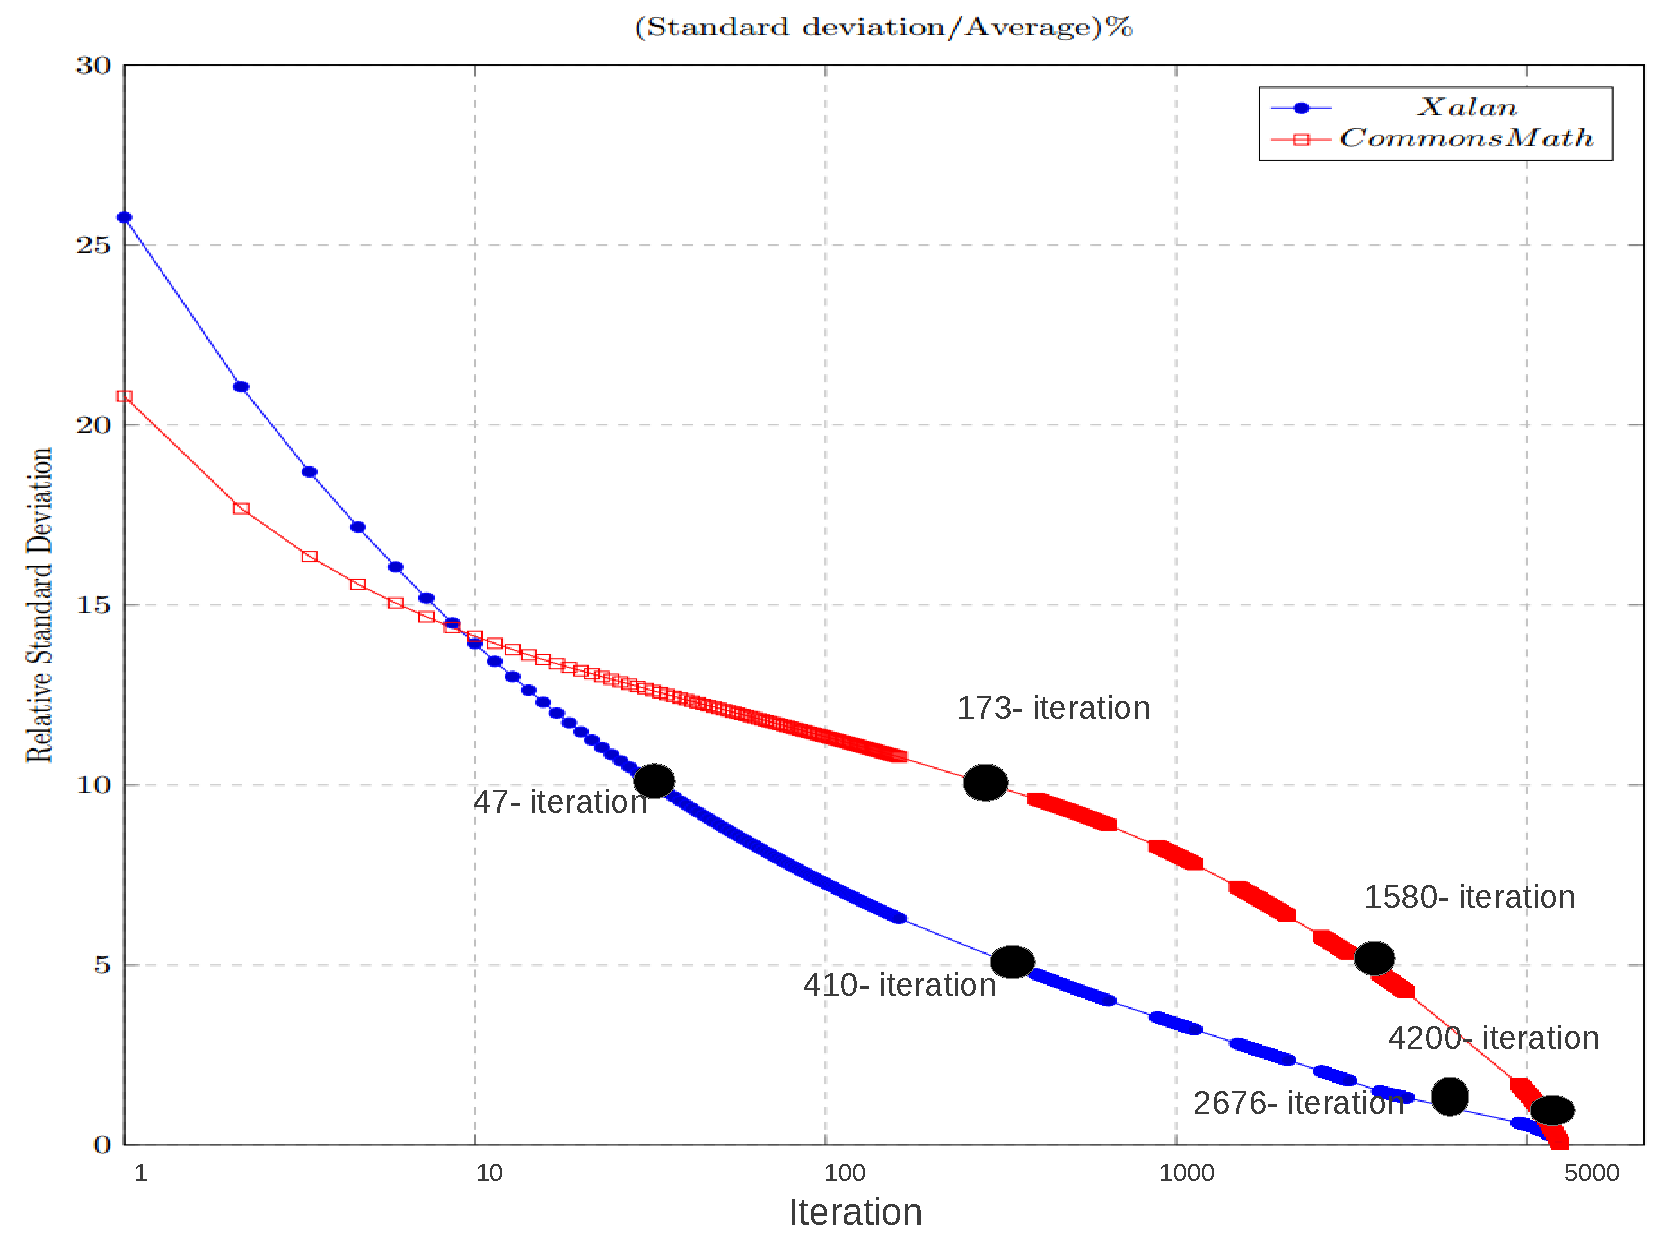
\includegraphics[width=0.45\textwidth]{performance/images/standard-deviation.pdf}
	\caption{Relative Standard Deviation vs. Sample Size}	
	\label{fig:motiv-math}	
	
\end{figure}

In this section, we provide preliminary study results to motivate prioritization of performance regression tests, due to high cost of executing the same test case for many times for performance regression testing. In particular, modern mechanisms in hardware and software often bring in random factors impacting performance. Some well-known examples are the randomness in scheduling cores and buses in multi-core systems~\cite{MultiCoreRandom}, in caching policies~\cite{CacheRandom}, and in the garbage-collection process~\cite{GBRandom}, etc. These factors interact with each other and amplify their effect so that the execution time of a test case may vary substantially from time to time. 

To neutralize such randomness, researchers or developers execute a test case multiple times and calculate the average performance~\cite{LiuCGO}. To better understand this requirement, we perform a motivating study (with more details on the project website~\cite{perfranker}) on the two open source projects used in evaluating our approach. In particular, we execute the test cases for 5,000 times, and randomly select samples with different sizes to calculate their standard deviation. In Figure~\ref{fig:motiv-math}, we show how the execution time's relative standard deviation (y axis) changes as the execution times (x axis) increase from 1 to 5,000. The figure shows that the average relative standard deviation with sample size 1 is over 20\% in both projects. In other words, if only one execution is used, the recorded execution time is expected to have more than 20\% difference from the average execution time in the 5,000 executions. Note that 20\% is a very large variance because 10\% performance enhancement is typically considered significant, and techniques incurring over 10\% overhead are often considered too slow for deployment purposes~\cite{DoubleTake}. The figure also shows that 173 and 47 executions are required to achieve relative standard deviation less than 10\% for Apache Commons Math and Xalan, respectively. Executing the whole test suite for many times can be prohibitively expensive, calling for prioritization of performance regression tests, as targeted by our approach. 


%The number of executions to acquire precise performance measurement may vary from scenario to scenario, and there is not a comprehensive study for it. In this paper, to understand how many executions are required to achieve precise result for our evaluation settings (i.e., performance testing of Java Projects on a state-of-the-art multi-core server), we performed a motivation study on the two test suite of our evaluation subjects: Apache Commons Maths and Xalan. 

%\textbf{Study Design.} For each project, we execute the test suite for 5,000 times on a quiet\footnote{``Quiet'' means that no other user process is running on the server.} DELL X630 server with 32 cores and 256GB memory. From the executions, for each test case, we recorded its execution time as a sequence with 5,000 data points\footnote{To avoid potential noises such as test-case loading or IO blocking, we removed the outliers that are beyond 2 times of standard deviation, which is a standard data purification process~\cite{}, and removed 0.9\% data points on average.}. In our study, we define ~\textit{Sample Size} as the number of iterations a test case is executed, and ~\textit{Sample Performance} as the average execution time calculated from the executions. For a small sample size (e.g., 1), the sample performance from different samples tends to have larger standard deviation, and when the sample size gets larger, the standard deviation among samples tends to get smaller, and our goal is to find the sample size that can lead to small enough standard deviation. 
%
%For each sample size $i$, we use all the sub-sequences with length $i$ of the original data-point sequence whose length is $N$\footnote{The value of $N$ is slightly smaller than 5,000 due to data purification.}
%
%Specifically, if the $k^{th}$ data point in the original data-point sequence is denoted as $ex(k)$, the first sample, the $k^{th}$ sample, and the last sample in the set will be:
%
%\begin{multline}
%sample(i, 1) = \{ex(1), ex(2), ...., ex(i)\}\\
%sample(i, k) = \{ex(k), ex(k+1$ $mod$ $N), ...., ex((k+i)$ $mod$ $N)\}\\
%sample(i, N) = \{ex(N), ex(1), ...., ex(i-1)\}\\
%\end{multline}
%
%Therefore, our sample set for sample size $i$ can be viewed as executing the test case for $i$ times from any start point in the original execution sequence. Based on these sample sets, if we denote the sample performance of $sample(i, k)$ as $perf(i, k)$, the relative standard deviation for sample size $i$ can be calculated as follows. 
%
%\begin{equation}
%Var(i) = \frac{Std(\cup{k=1}{N}{\{perf(i, k)\}\}})}{\Sigma{k=1}{N}{ex(k)}/N}
%\end{equation}
%
%In the formula, to normalize the standard deviation for different test cases and projects, we divide it with the average execution time of the test case for all $N$ executions. Therefore, we actually use the average execution time of the 5,000 executions to approximate the ideally precise execution time. It should be noted that, 5,000 is much larger than 10 to 100 which are common used in performance related research efforts in literature~\cite{}~\cite{}, so we believe that the approximation should be reasonably accurate.  For the sample sizes from 1 to 5000, we draw the trends of relative standard deviation (average for all test cases)
%\textbf{Study Results.} 


% 1,580 and 406 executions are required to achieve relative standard deviation less than 5\%. 



%in which horizontal axes represent sample sizes in log scale and vertical axes represent the relative standard deviation. 


%It should be noted that, our study has some limitations such as the purification of execution-time outliers which may exist in the real world testing, and the fact that sample sets are not independent with each other because there are overlaps between neighboring sample sets (e.g., $sample(i, 1)$ and $sample(i, 2))$. However, these two limitations will both reduce the observed relative standard deviation, indicating that we actually provided a lower bound of relative standard deviation over sample sizes. Therefore, as a motivation study, it show that we do need several hundred executions to confirm a performance regression around 10\%. Based on this fact, the prioritization of test cases is very helpful, because we can focus the highly prioritized test cases, and execute them for more times to better confirm perform regressions. 





%We can see that at first iteration average deviation from ideal is 20.79\% and reduced to 5\% with 1580 iteration. Finally the overall variance decreased to 1\% with iteration 4200. Furthermore, deviation decreases sharply from 20\% to 10\% with 173 times of execution whereas reduction from 10\% to 5\% take 1407 iteration. So we can say that large number of iteration of execution of test case are needed to get a stable execution time of a performance test case. A small extent of performance degradation may result in severe consequence motivate us that running performance test needs more time and resources. It is hard for a developer to understand performance impact with few runs.\\


%In the evaluation of techniques for compilers and systems, to reduce some randomness, researchers sometimes choose to turn off some features, such as doing garbage collection at fixed time point. However, 

%{\fontsize{7}{7}
%\begin{multline}
%\begin{gathered}
%Average = Avg(1,2,3,...,5000)\\
%Var(i) = \frac{ Std( Avg(1,2,...,i),...,Avg(5000,1,...,i-1))}{Average}\\
%Iteration(i) = \frac{ \sum \limits_{k=1}^{alltest} Var(i)}{alltest}
%\label{eq:eq-motivation}
%\end{gathered}
%\end{multline}
%}





%We run real test cases and captured average execution time of two popular open source project apache common math and xalan. \textbf{Common math}:  We chose 2703 test cases which are affected by code changes from a collection 3900 test cases and each of test cases  exercise 5000 time and record their execution time. In the formula ~\ref{eq:eq-motivation} function Avg and Std corresponding to average and standard deviation. For iteration-1, it becomes {\fontsize{7}{7}\[ Var(1) = \frac{Std(1,2,3,...,5000)}{Average}\]} which is fraction of standard derivation of 5000 data and average of 5000 data. The value of Var(1) represents how far the deviation is from the ideal case with a single iteration.For iteration-2, it becomes {\fontsize{7}{7} \[Var(2) = \frac{ Std( Avg(1,2), Avg(2,3),...,Avg(5000,1))}{Average}\]} where each data of standard deviation is average of 2 data which means that 2-iteration on the average how much deviate from ideal case. For iteration-5000, it becomes {\fontsize{7}{7}\[Var(5000) = \frac{ Std(Avg(1,2,...,5000),...,Avg(5000,1,...,4999))}{Average}\]} where each data of standard deviation is average of 5000 data which means Var(5000) value equals to zero that we considered as ideal or base case. According to the formula~\ref{eq:eq-motivation}, we generate a graph in the figure ~\ref{fig:common-math-motiv} 

\section{Approach}
\label{sec:approach}

In this section, we introduce our test prioritization approach in detail. In particular, we first present the overview of our approach, major technical challenges, and our performance model. After that, we introduce performance-impact estimation of a code commit based on our performance model, including method-execution-time estimation, and method-invocation-frequency estimation based on collection-loop correlation and iteration-count inference.


\subsection{Overview}

%To prioritize performance test cases, the core difficult

%The objective of PerfChecker is to examine a code commit content and determine the cost of a change, and then rank the performance test case on basis of a change performance impact cost which helps to reduce the cost in performance regression testing. Profiler takes the base version code and statically modifies the code in order to extract profile information. Run all the performance test case and store method execution time, execution frequency and loop counter in profile database.Profile database also store JDK library method's execution summary. 

\begin{figure}
\centering
	
	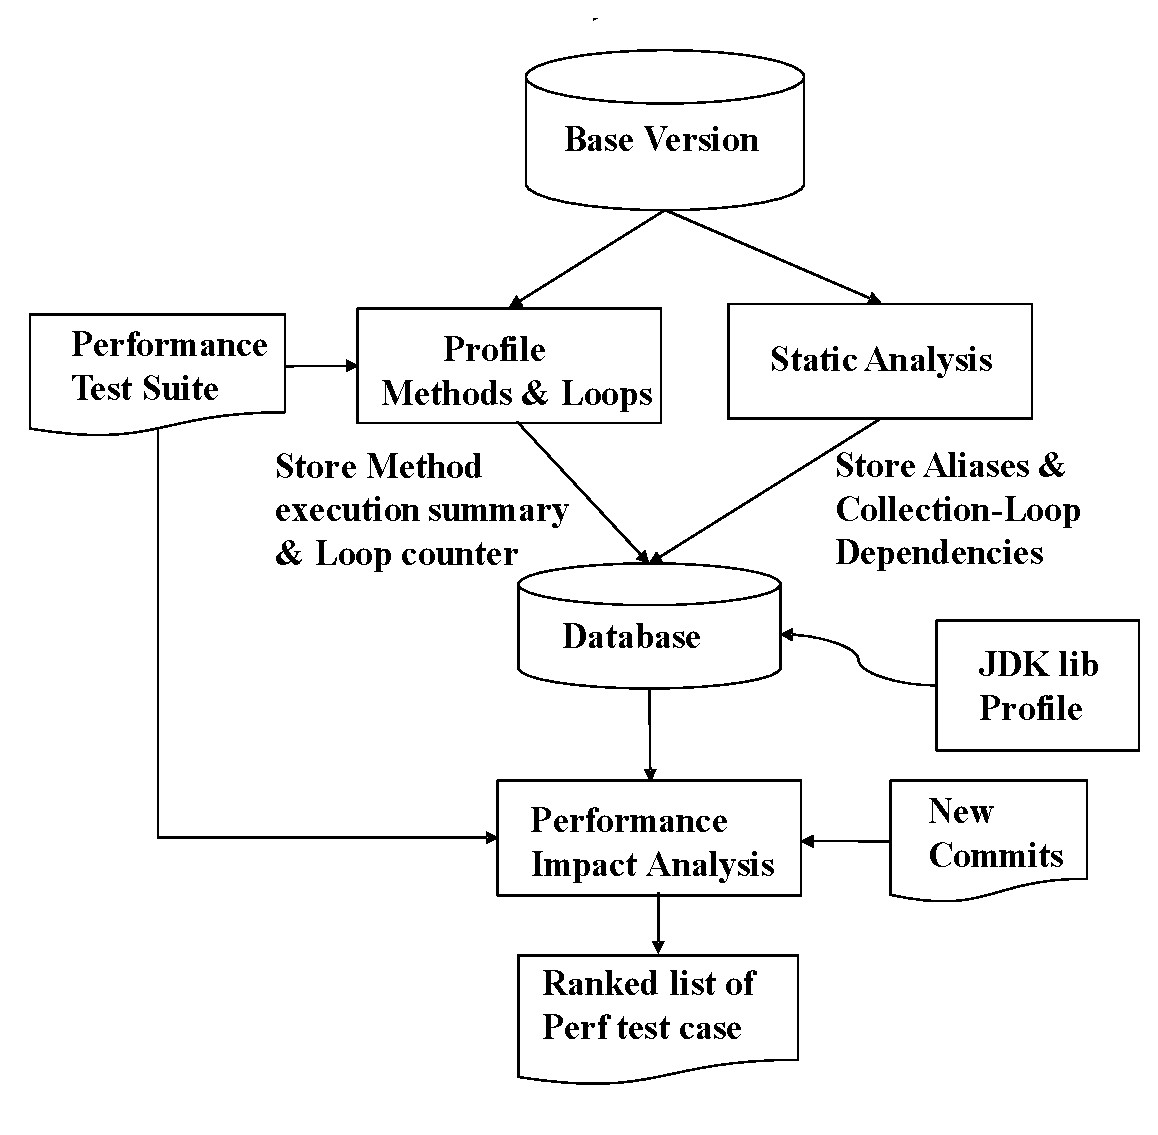
\includegraphics[width=3.5in, height=3.5in]{performance/images/Workflow2.pdf}
	\caption{Workflow of Our Approach}	
	\label{fig:approach-workflow}
		
\end{figure}

Figure~\ref{fig:approach-workflow} shows the workflow of our approach. The input to our approach includes the project code base, its code commits, and performance test cases. The output of our approach is an ordered list of performance test cases. The first step of our approach is to  profile the base version of the project under test. During the profiling, for each test case, we record the dynamic call graph as its original performance model. We also record average execution time and frequency of methods, and iteration counts of all loops. At the same time, we statically analyze the base version to gather dependencies between loops and collection variables, as well as aliases among collection variables. When a new code commit comes, we conduct performance impact analysis to estimate its performance impact on all test cases, and prioritize test cases accordingly. 


%Another component is Alias analyzer which statically analyze the source code loop controlling variable, array and collection with their alias and store their information in database. Diff generator produce diff of each committed code into the repository. Parser parses information regarding the changed files, lines and types (add, delete) from the generated diff file content. Filter prunes out insignificant change such as stylish change or renaming. If the changes are significant, the commit will be considered to fed to the performance impact analyzer. Performance impact analyzer analyse the cost of the change by constructing CFG of the modified method and integrating the profile information from the database into the call graph of the test case. At the final stage it produce a sorted list of test case according the cost performance impact score. 



 
 
%The challenge is how to estimate the cost about performance impact of each of test case after a change without actually running the software.We first briefly describe the input-output of our approach and major component. 

%Although it is straightforward to prioritize test cases based on the code commit's performance impact on them, 

\textbf{Technical Challenges.} Performance impact analysis is the core of our approach. Although we focus on collection-intensive software, it is still challenging to conduct performance impact analysis, facing three major technical challenges:

\begin{itemize}

\item Challenge 1. A code commit may include any type and scope of code changes, from one-line revision, to feature addition and interface revision. Therefore, there is a strong need of a unified and formal presentation for code commits.  

\item Challenge 2. A code commit may contain newly added code, especially new loops. No execution information of such code is available, but given that loops can have high impact on performance, there is a strong need of estimating the code commit's execution time and frequency.
 
\item Challenge 3. Even if the execution time of changed code in a code commit has little impact on performance, the code commit may include changes on collection variables, eventually affecting the performance of unchanged code. 

%In our paper, we refer such performance changes as \textit{side performance impact}. 

\end{itemize}

To address Challenge 1, we present a code commit as three sets of methods: added methods, revised methods, and removed methods. As our performance model is based on the dynamic call graph, any code commit can be mapped to a series of operations for method addition, removal, and replacement in the performance model. To address Challenge 2, we leverage the recorded profiling information of the base version as much as possible. Specifically, if an existing method is invoked in the newly added code, we can use the recorded execution time of the existing method as its execution-time estimation for this new invocation. Furthermore, as discussed in Section~\ref{sec:intro}, we use collection variables as bridges to estimate iteration counts of new loops from those of existing loops. To address Challenge 3, we track all the element-addition and element-removal operations of collection variables in the newly added code, and estimate the size change of collection variables from the iteration count of their enclosing loops. This new size is used to update the iteration counts of loops depending on the changed collection variables. 

%Note that, the execution time of added and removed methods can affect existing test executions only through revised methods, where invocations to them are added and removed. %For each revised method, based on the performance model in Section~\ref{subsec:model}
%we estimate the execution time of the pre-commit version and post-commit version, respectively, and estimate the performance impact of a revised method as the execution-time difference between its pre-commit version and post-commit version. Then, the directly performance impact of a code commit can be calculated as the performance impact sum of all revised methods, together with side performance impact. 



%and if a newly added loop depends on an existing collection variable, 

%we can use the recorded size of the collection variable to estimate the number of iterations of the loop. The detailed process of estimating direct performance impact is presented in Section~\ref{subsec:direct}. 



%their new value ranges in the new version according to the iteration number of the writing operations. Then, for each collection variable $v$, if there is any loop $l$ depending on $v$, we calculate the side performance impact of $l$ with $v$'s new value range and sum up side performance impact of all such loops. The detailed process of estimating side performance impact is presented in Section~\ref{subsec:side}.

Since we focus on collection-intensive software, we consider only loops whose iteration number depends on collection variables, e.g., variables of array type, and other collection types defined in Java Utility Collections. Note that there are also some loops whose iteration number depends on simple integers, such as a loop to sum up a numbers from $i$ to $j$, but such loops are not common in collection-intensive software, and our evaluation results show that our approach is effective on both data-processing software (Xalan) an mathematics software (Apache Commons Maths). 

%The rationale behind this design decision are (1) according to literatures~\cite{}~\cite{}, most performance issues are related to loops; and (2) most loops in programs are for manipulating iterative data structures (i.e., collection variables).  


%This is a limitation of our performance impact analysis, b ut 
  
\subsection{Performance Model}
\label{subsec:model}
\begin{figure}[t]
\centering
  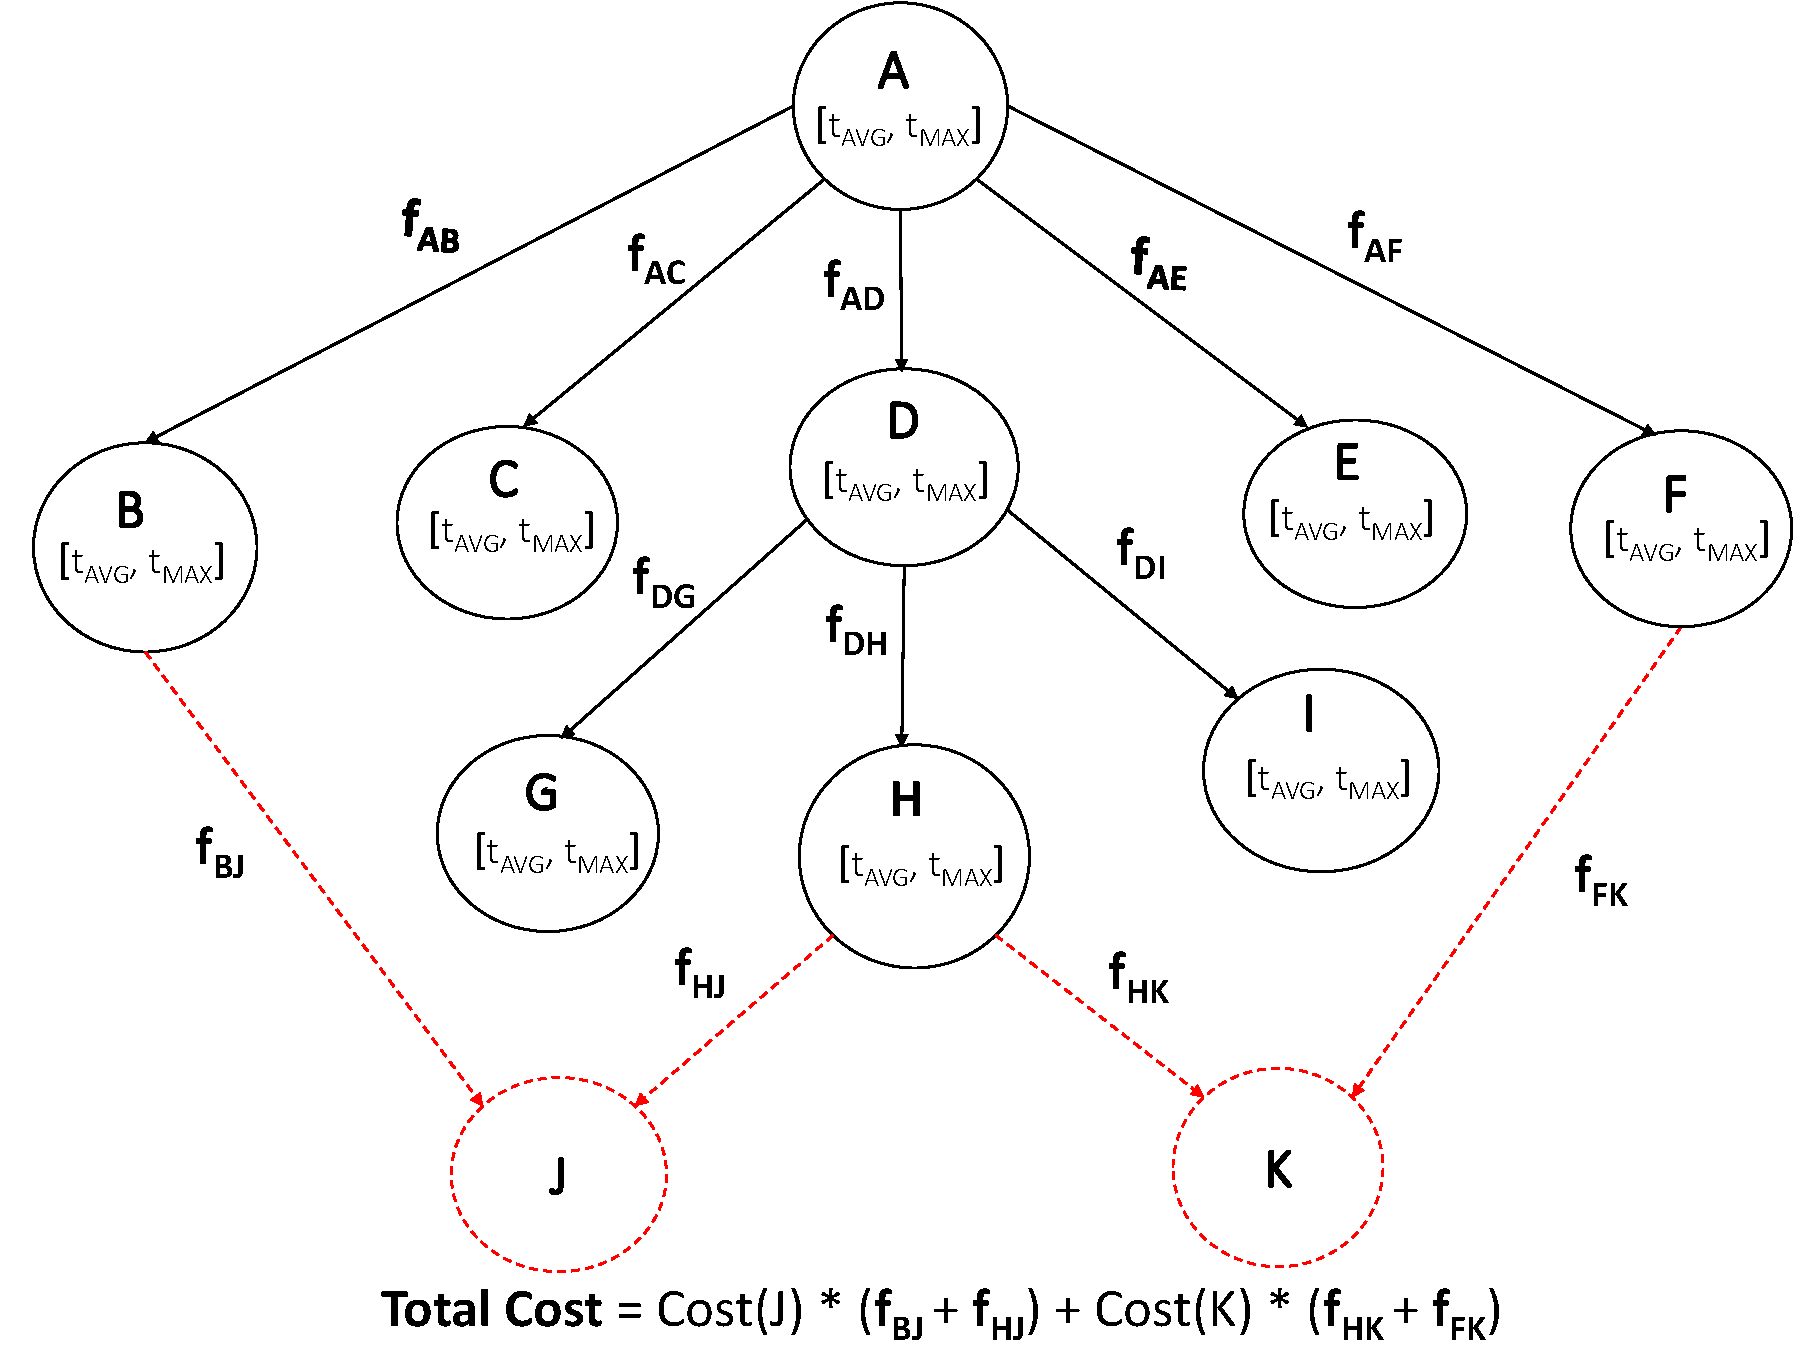
\includegraphics[width=4in, height=3in]{performance/images/performance-model.pdf}
  
   \caption{An Example Performance Model}	
    \label{fig:performance-model}
   
 \end{figure}

In this subsection, we introduce our performance model to break  down execution time of a test case to all the methods invoked by the test case. The basic intuition behind our model is that the execution time of a method invocation $M$ is the execution-time sum of all method invocations directly invoked in $M$, together with the execution time of instructions in $M$. Since most basic operations in Java programs are performed by JDK library methods (e.g., a string concatenation), the latter part is typically trivial compared with the former part, so our performance model ignores instructions in $M$ itself, but focuses only on methods that $M$ invokes. 

%Specifically, for each test case, our performance model is based on the dynamic call graph of the test case. So the nodes of the graph are method bodies, and the edges are invocations. In the graph, we record two attributes: invocation frequency, and average execution time. For example, on the directed edge from method $A$ to method $B$, we record the average number of invocations from $A$ to $B$ in each invocation of $A$, and on the node $B$, we record the average execution time of $B$.  

We illustrate our model in Figure~\ref{fig:performance-model}, where each node represents a method and each directed edge represents an invocation relation. Here each node annotated with label $t_{avg}$, which represents the average execution time of a method. Each edge in the graph is labeled with $f_{AB}$, which represents the invocation frequency of method B from method A. Given a code commit, the performance model of the post-commit version can be acquired by adding and removing nodes and edges to the original performance model. For example, in Figure~\ref{fig:performance-model}, method $D$ is a revised method and it now calls (1) method $G$, which it originally calls, (2) $E$, which is an existing method in the base version, and (3) $H$, which is a newly added method. With the average execution time and invocation frequency of all invoked methods in $D$, we are able to calculate an execution-time estimation for revised method $D$. The new execution time at $D$ can be propagated upward to its ancestors, until the main method is reached and a new estimation of the whole program's execution time can be made. 


% $m\textsubscript{K}$ are changed and they are called from multiple context $m\textsubscript{B}$,$m\textsubscript{G}$  and $m\textsubscript{H}$. So the total cost is calculated from the modification cost of method $m\textsubscript{J}$  and $m\textsubscript{K}$ by multiplying the frequency  $f\textsubscript{BJ}$,$f\textsubscript{GJ}$,$f\textsubscript{HK}$ and $f\textsubscript{GK}$. Finally, The cost is propagated from child to parent in the graph.

\subsection{Performance Impact Analysis}
\label{subsec:direct}

The basic idea of performance impact analysis is to calculate the  execution-time change of each revised method $M$ in the code commit. Then, through propagating the execution-time change to $M$'s predecessors in the performance model, we can calculate the execution-time change of the whole test case at the root node. 

%We focus only on revised methods because added and removed methods may affect software performance only through revised methods (i.e., by adding or removing method invocations).

We realize this idea in three steps. First, for each revised method, we extend the performance model to either add it and/or some of its callees (and transitive callees). Second, we estimate the execution-time change of each method in the new performance model. Third, we estimate the invocation frequency on the edges of the new performance model. We next introduce the three steps in details.



\subsubsection{Model Extension}
\label{subsub:findInvoke}

For each revised method, we add its direct and transitive callees (e.g., methods $E$ through $K$ in Figure~\ref{fig:performance-model} for the revised method $m_D$) into the performance model, if they do not already exist in the model. In this recursive process, we terminate the extension of a method node if it is an unrevised method existing in the base version, a JDK library method, or a method whose source code is not available. Since we use one base version for a series of code commits, a revised method (and even some of its predecessors) may not exist in the base version because they are added after the base version. In such a case, we transitively determine $M$'s predecessors (callers) until we reach methods in the base version. For example, if $C$ and $D$ in Figure~\ref{fig:performance-model} are added between the base version and the code commit under analysis, we determine that $D$ is invoked by $B$ and $C$, and $C$ is invoked by $A$, so that we add $C$ and $D$ to the performance model. 

When the new code version of the revised methods is available, we  
statically determine the direct and transitive callers and callees for the revised method, and one remaining challenge is to resolve polymorphism, where one method invocation may have multiple targeted method bodies. Although it is straightforward to apply off-the-shelf points-to analysis, since we have the profiling information of the base version, we make use of the information to acquire a more precise call graph. Specifically, if a method invocation is not involved in the method diff (i.e., the method invocation can be mapped to the same method invocation in the base version, such as $G$ in Figure~\ref{fig:performance-model}), we assume that its target is not changed and we use the same targeted method body as recorded for the base version. Otherwise, we apply points-to analysis~\cite{Spark} in Soot~\cite{Soot} to find the possible targeted method bodies for the method invocation. When a method invocation is mapped to multiple method bodies, we add all bodies to the new performance model, and we divide the estimated frequency of the method invocation by the number of possible targets to attain the invocation frequency of each target. 

%Analyzing the new code version of the revised method, it is straightforward to build a partial call graph with it as the root node. Since  resolve polymorphism, we use the following heuristic. 

%Therefore, by listing all the added and deleted methods and their execution time summary will provide an estimate of 

%So combining the profiling information and control flow analysis together may provide accurate estimate of cost of modified method.

%Estimate the cost of a modified method need to identify all the changes inside the method which are added and deleted.




\subsubsection{Execution-Time Change of Method Bodies}
\label{subsub:findExetime}

The method bodies invoked from a revised method fall into three  categories. The first category is removed method bodies. Their execution-time data are recorded in the performance model of the base version, and their new execution time is estimated as 0.

The second category includes method bodies already existing in the performance model of the base version. Such method bodies include both those defined in the source code and those defined in the JDK library, or those without source code. For existing method bodies, we simply use the recorded average execution time in the base version as their estimated average execution time. For bodies of JDK library methods, we profile Dacapo~\cite{dacapo} to acquire the average execution time of those common JDK library methods. For methods without source code or those not invoked by Dacapo, we use the average execution time of all method bodies in the profile as their estimated execution time, as we have no further information. Note that when a method from the second category is added to the performance model, its original execution time is set as 0.

The third category includes newly added method bodies in the source code. \textit{Note that such method bodies include both those added to the source code in the code commit and those added in any other code commits between the base version and the code commit under analysis.} They also include method bodies defined in libraries but are newly reached due to code revisions from the base version to the new version. For a newly added method body (such as $H$ in Figure~\ref{fig:performance-model}), as discussed in Section~\ref{subsub:findInvoke}, we extract all its callee method bodies, and add them to the performance model (such as $J$ and $K$ in Figure~\ref{fig:performance-model}), and then we calculate its execution-time change using our performance model.

%If an added callee method body still belongs to category-2, then we can iteratively extract its callee method bodies. The extraction process will terminate when all the newly added callee method body either belongs to category-1, or is defined in Java SDK. 



%Changes inside a method normally consists of addition and deletion of existing method call or addition of newly method call. 
%Profile all the performance test case and store their average execution time  will provide the cost of existing method call.
%A newly added method also consists of existing method, JDK library call and newly added method. So profiling JDK library function call
%also helpful to estimate the cost of newly added method. if no information available then statically analyse the change and assign the cost based on the existence of loop and hot api call like database, storage and network.
 
\subsubsection{Invocation Frequencies of Method Bodies}

Given a newly added or revised method $m_x$, for each method $m_y$ that is directly invoked in $m_x$, we estimate the invocation frequency of $m_y$ in $m_x$ (denoted as $fq(m_x, m_y)$) to apply our performance model on the new version. Our estimation technique is based on the control flow graph of $m_x$ and the average iteration counts of loops in $m_x$. Specifically, for any code block $b$ in $m_x$, we use $fq(b, m_y)$ to denote the invocation frequency of $m_y$ from $b$ for each execution of $b$. If $b$ is a basic block without branches and loops, $fq(b, m_y)$ is exactly the number of invocation statements to $m_y$ in $b$; such number can be easily counted statically. Then we calculate $fq(m_x, m_y)$ by applying the inference rules for sequential, branch, and loop structures in Formulas~\ref{equa:seq}-\ref{equa:loop} below recursively on the code blocks of $m_x$:

   
\begin{equation}
\label{equa:seq}
fq([\text{$b_1$; $b_2$}], m_y) = fq(b_1, m_y) + fq(b_2, m_y)
\end{equation}
\begin{equation}
\label{equa:branch}
fq([\text{if() $b_1$ else $b_2$}], m_y) = Max(fq(b_1, m_y), fq(b_2, m_y))
\end{equation}
\begin{equation}
\label{equa:loop}
fq([\text{while$_i$ () $b$}]) = fq(b, m_y) \times C(loop_i)
\end{equation}

In the inference rules, the only unknown parameter is $C(loop_i)$, which denotes the average iteration count of the i$^{th}$ loop in $A$. As an example, given the control flow graph in Figure~\ref{fig:cfg-sample} of m$_x$, for any $m_y$ that $m_x$ invokes, $fq(m_x, m_y)$ can be estimated as in Formula~\ref{equa:example}.

\begin{figure}
\centering
	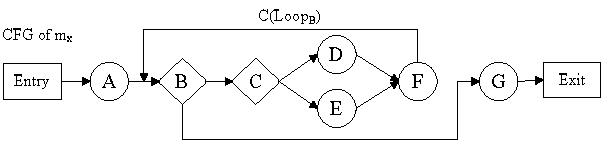
\includegraphics[width=3.5in, height=1in]{performance/images/cfg-new.pdf}
	
	\caption{An Example Control Flow Graph}	
	
	\label{fig:cfg-sample}
\end{figure}


%Ifwe try to estimate $freq(A, B)$ as a function of average iterations in $A$

%Generally, a change set may introduce performance regression in two ways: one case is the change itself in the hot path of execution and another case is that changes modifies some control variables which result some part of code executing very frequently. We can estimate how frequently the method executing in two ways: Loop correlation and Collection propagation. %Generally the changes inside a method does not lie in a single execution path. Control flow analysis of a modified method helps to identify all the paths inside the method and the changes in the path. 

   
\begin{multline}
\label{equa:example}
fq(m_x), m_y)=fq(A, m_y) + (Max(fq(D, m_y), fq(E, m_y))\\ + fq(F, m_y)) \times C(Loop_B) + fq(G, m_y)
\end{multline}
\vspace{-0.5cm}

%shown a simple CFG of a change of a modified method where each node represents a block of CFG and each annotated with cost which is sum of all the method execution time inside the block. There are two path from node B to node F.  $Cost\textsubscript{BDF}$ is the cost of path $BCDF$ and $Cost\textsubscript{BEF}$ is the cost of path $BCEF$. So the maximum cost will the maximum of this two path multiplied by the loop counter which is the execution time of changes in the method.


 
%\subsection{How to decide How many times a method will execute}
%Generally, a change set may introduce performance regression in two ways: one case is the change itself in the
%hot path of execution and another case is that changes modifies some control %variables which result some part of code
%executing very frequently. We can estimate how frequently the method executing in two ways: Loop correlation and Collection propagation.  

\subsection{Loop-Count Estimation with Collection-Loop Correlation} 

With the estimation of invocation frequency, the only remaining unknown parameter in the performance model of the new version is the loop count of all loops. If a loop exists in the base version and is not affected by the code commit, we directly use the recorded profile from the base version to acquire the iteration count. Two more complicated cases are (1) when a new loop is added, and (2) when the code commit affects the iteration count of an existing loop. Here is our insight: for collection-intensive software, we can construct the correlation between collection sizes and loop counts, and use iteration counts of known loops to infer that of unknown loops, as well as a code commit's impact on iteration counts of known loops. 

\subsubsection{Correlating Loops and Collections} In particular, we consider the following two types of dependencies between loops and collection variables:

\begin{itemize}
	\item Iteration Dependency. A loop $L$ is iteration-dependent on a collection variable $v$ if $L$'s loop condition depends on the size attribute of $v$.
	\item Operation Dependency. A collection variable $v$ is operation-dependent on a loop $L$ if there exists an element addition or removal on $v$ in $L$.
	\vspace{-0.15cm}
\end{itemize}

To identify iteration dependencies, for a For-Each loop (e.g, \CodeIn{for(A a : ListOfA)}), we simply consider that the loop is iteration-dependent on the collection variable being iterated via the loop. For other loops, we use standard inter-procedural data flow analysis~\cite{SootIFDS}~\cite{IFDS} to track data dependency backward from the loop condition expression, until we reach a size/length attribute of an array or a known collection class from the Java Collection Library. To make sure that the collection size is comparable with the loop count, we consider only two types of data dependencies: (1) direct assignment (e.g., \CodeIn{a = b;}), and (2) addition or subtraction expression with one operand as constant (e.g., \CodeIn{a = b.size() - 1}). 

To identify operation dependencies, for each loop $L$, we check its body for element-addition and element-removal operations on collection variables. For any other method invocations in the loop, we recursively go into the body of each invoked method to further look for such operations. However, we do not consider nested-loop blocks in $L$ or a method invoked from $L$, because such blocks are dependent on their direct enclosing loop. For example, in Figure~\ref{fig:operationDepend}, collection variable $v$ is operation-dependent on Loop$_A$, but $w$ is not (it is operation-dependent on Loop$_B$). 

\begin{figure}
\centering
	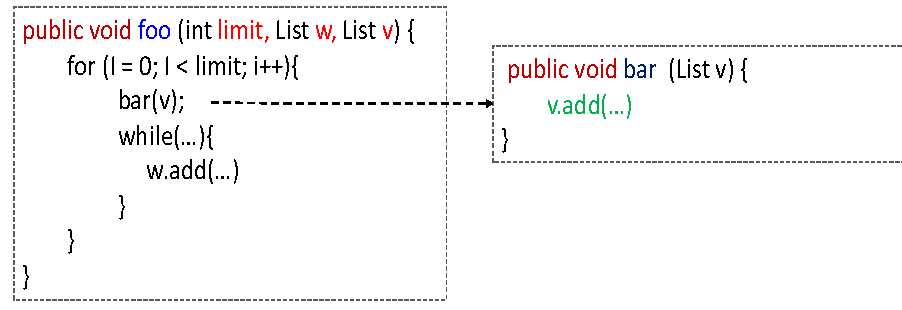
\includegraphics[width=3.5in, height=1.3in]{performance/images/operationDepend.pdf}
	
	\caption{Code Sample of Operation Dependency}	
		
	\label{fig:operationDepend}
\end{figure}




After identifying these two types of dependency relations, we further apply points-to analysis~\cite{Spark} to identify alias relations among collection variables. Note that in our analyses we consider only variables of known collection classes from the Java Collection Library. User-defined collections are also common. However, since we use inter-procedural analysis for identifying both types of dependencies, as long as the user-defined collections extend or wrap Java-Collection classes from the Java Collection Library, we are able to handle these user-defined collections by building dependencies directly on the Java-Collection variables inside them. Also note that  we identify all dependencies and alias relations on the base version and record the results so that we need to re-analyze only the revised/added methods when a code commit comes. 

\vspace{-0.2cm}
\subsubsection{Iteration-Count Inference}


With the dependencies identified among collections and loops, when a new code commit comes, we use Algorithm~\ref{alg:infer} to infer the iteration count of new loops and update the iteration count of existing affected loops. 

In the algorithm, we use a work queue to iteratively update sizes of collection variables and loop-iteration counts (stored in $lCount$), and we use the combined map of $MapI$ and $MapO$ to transit between collections and loops. In particular, as shown in Lines 6-11, we update the iteration count of each loop at most once, to avoid infinite update process caused by cyclic dependency (the more in-depth reason is that we use numbers to represent iteration counts, which are not in a bounded domain). In the end, we remove collection variables from $lCount$ to retain only the loops in the map.

\setlength{\textfloatsep}{6pt}
\begin{algorithm}[t]
	\begin{algorithmic}[1]		
		\REQUIRE~~\\
		$MapO$ is a map from collection variables to loops\\
		$MapI$ is a map from loops to collection variables\\
		$lCount$ is a map from loops to iteration counts\\
		\ENSURE~~\\ updated $lCount$\\
		\STATE{$Q \leftarrow MapI.keys()$}
		\STATE{$Map \leftarrow MapO \bigcup MapI$}
		\WHILE{$Q \neq \emptyset$}
		\STATE{$top \leftarrow Q.pop()$}
		\FORALL{$val \in Map.get(top)$}
		\IF{$val \notin lCount.keys() $}
		\STATE{$lCount.add(val, lCount.get(top)$}
		\STATE{$Q.add(val)$}
		\ELSIF{$val$ is a collection variable}
		\STATE{$lCount.set(val, lCount.get(val) + lCount.get(top)$}
		\STATE{$Q.add(val)$}
		\ENDIF
		\ENDFOR
		\ENDWHILE
		\STATE{$lCount.removeAll(MapO.keys())$}
	\end{algorithmic}
	\caption{Iteration Count Inference}
	\label{alg:infer}
\end{algorithm}

\vspace{-0.2cm}
\subsection{Test Case Prioritization}
\vspace{-0.1cm}
Once our approach estimates the performance impact of the code commit on each test case, we can rank test cases according to their relative performance impact. We use the main method as the root for system tests and each test method as the root for unit tests. We consider both positive and negative effect on execute time as it is often also important for developers to understand whether and where their commit is able to enhance the software performance. 


%In the figure ~\ref{fig:approach_overviw_1}, changes in the method named as getNameSpaceURI is trivial to developer because the indirect cost is not visible to developer. We can see that grand parent in the calling stack has loop in nested which execute more that 8000 time in both case. As a result the changes happen in hot path introduce high cost. Furthermore, developer may not be aware of another loop in path which is a child method in calling stack. As a result average counter of this loop in each test case more than 144000 times which introduce performance regression. To address this problem we introduce call graph with calling context that will provide estimation how many times the modified method getNameSpaceURI could be called from parent. if we know the frequency of the method getNameSpaceURI in the context then it is easy to say how many time the newly added method will be invoked. Similarly the newly added child has a loop that correlated with array size provide the context how many time the methods inside loop will be executed. 

%\begin{figure}
%  \centering
%  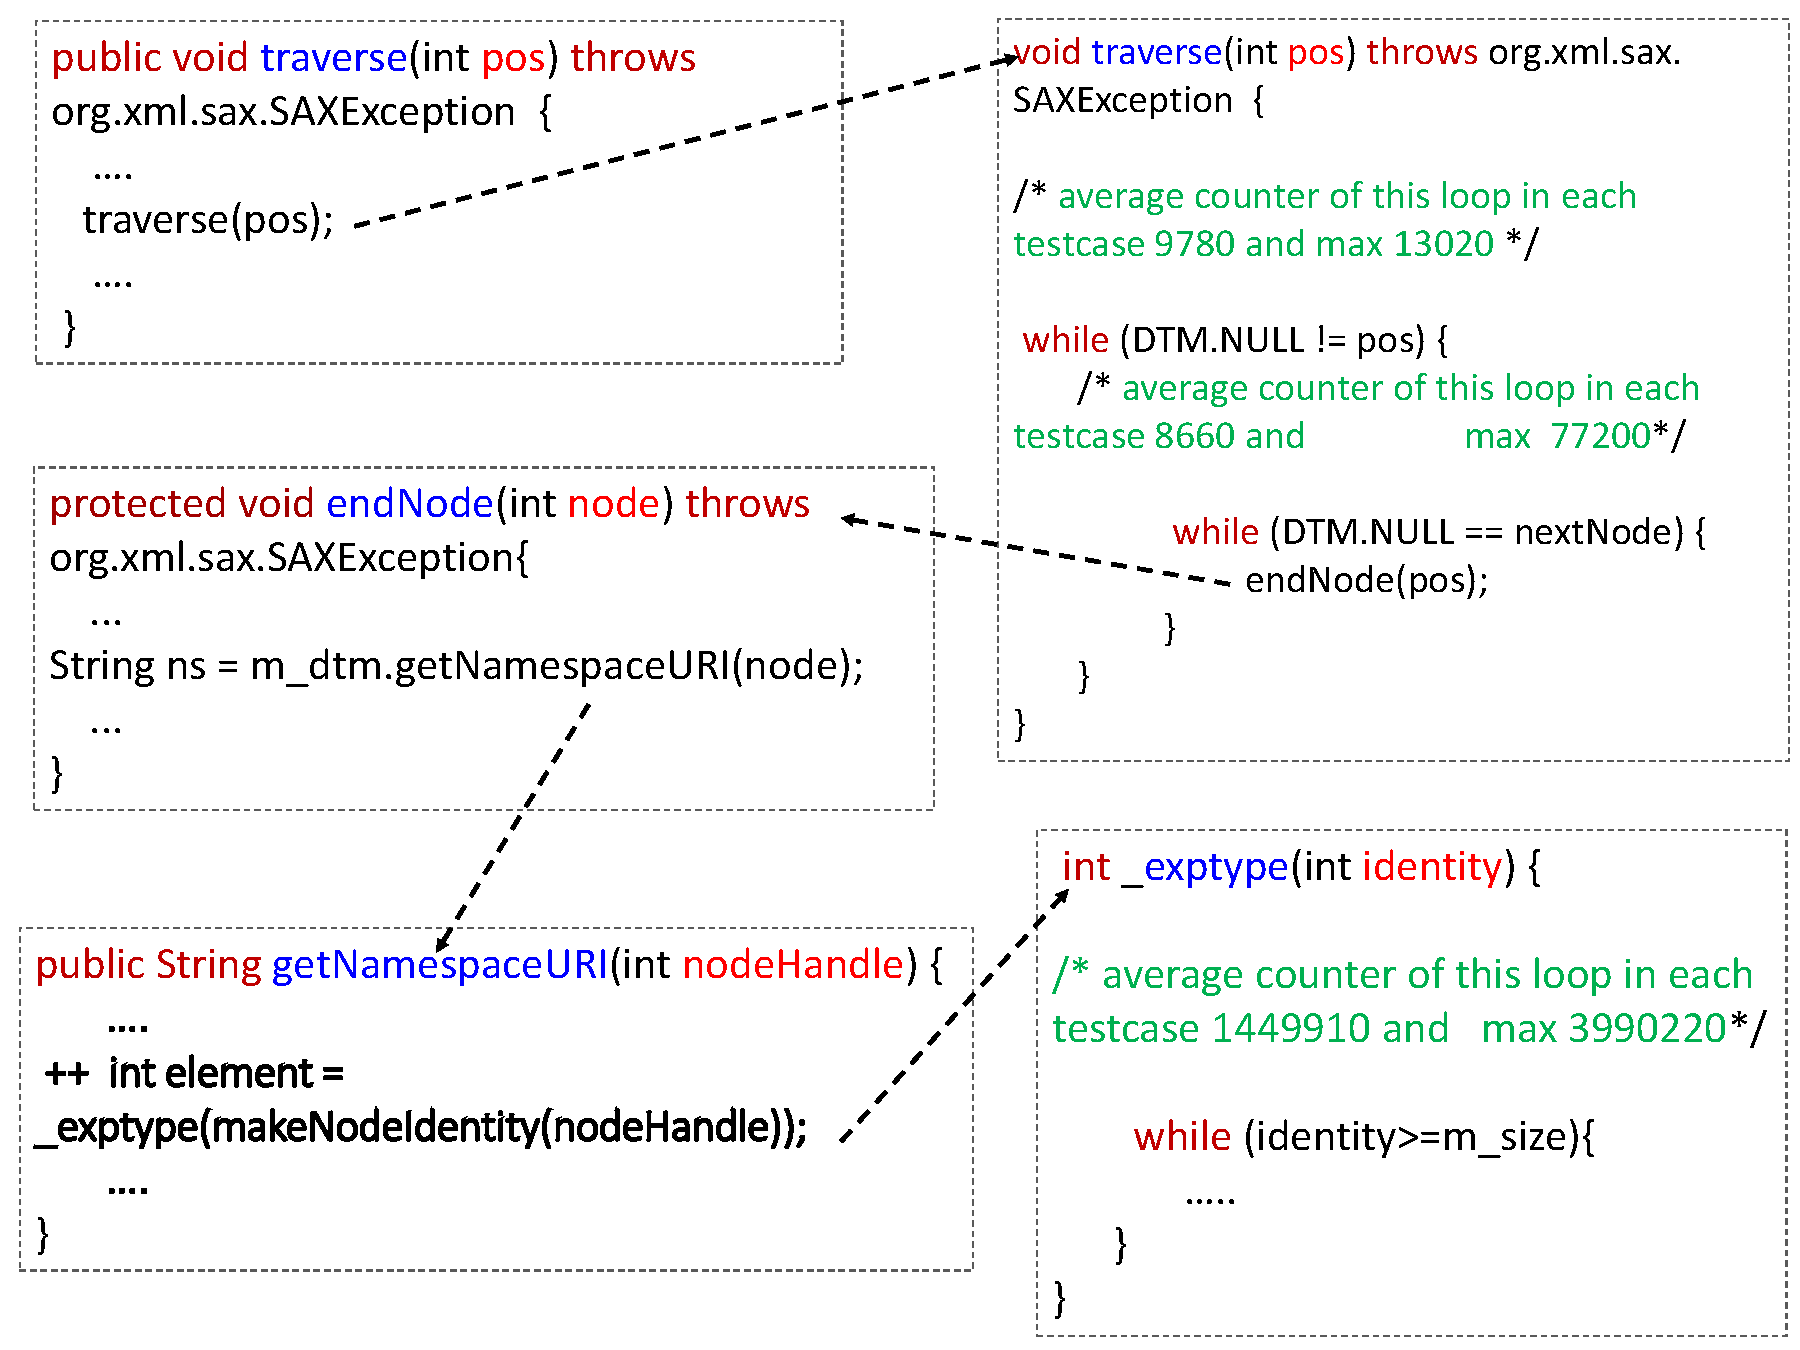
\includegraphics[width=\columnwidth,height=3in]{images/call-graph-example.pdf}
%  \caption{Overview of a change call graph in Xalan}	
%  \label{fig:approach_overviw_1}
%\end{figure}

%\subsubsection{Collection Propagation}
%The most common nature of loop in source code is iterate of over array or collections and changes inside loop introduce cost. 
%Generally, collection or array are propagated two ways: parameter passing and field variable. In the figure ~\ref{fig:approach_overviw_2} we can see that three different methods has loop that depends on the size of ArrayList and most
%importantly they are alias. if one of method loop counter is known then any new invocation of other method's loop counter can be predicted which will be helpful to estimate how many times the method under a loop will be called. So static analysis and alias analysis are important way to the solution of the problem.
%
%\begin{figure}
% \centering
%  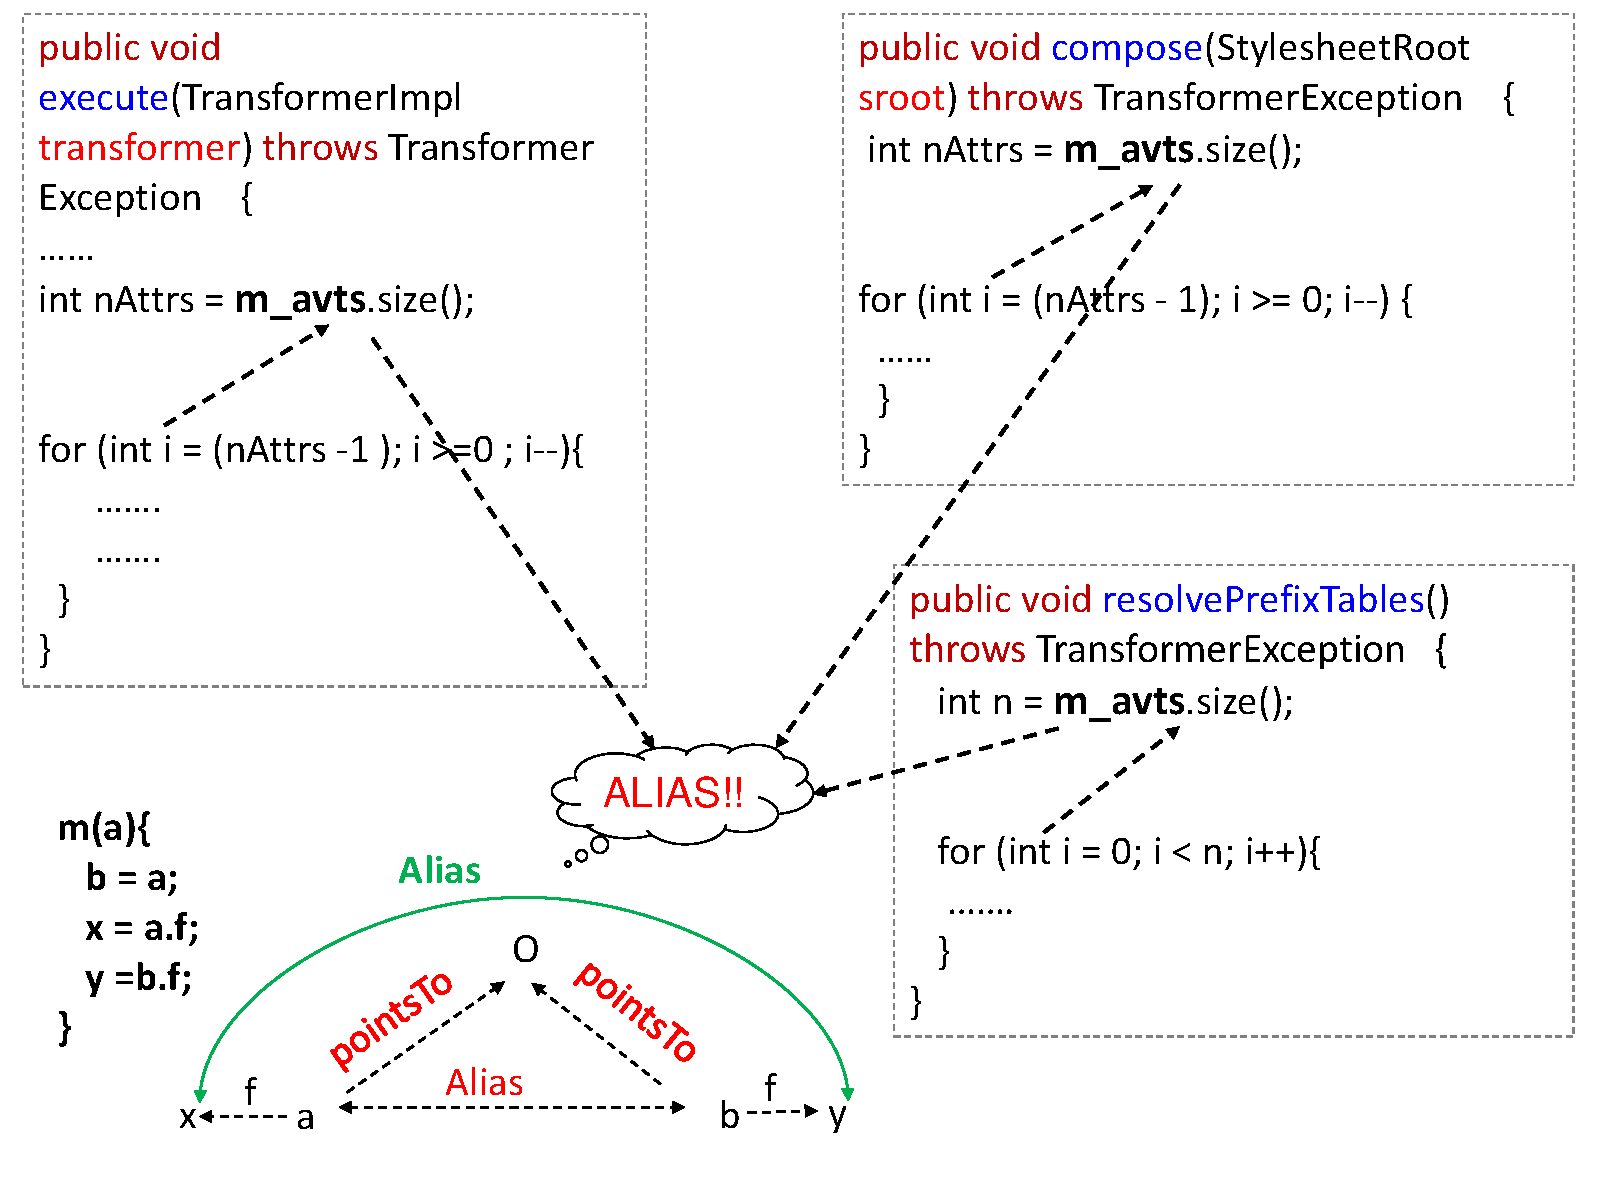
\includegraphics[width=\columnwidth,height=3in]{images/Alias-example.pdf}
%	\caption{Overview of a alias in Xalan}	  
%  \label{fig:approach_overviw_2}
%\end{figure}
%
%
%\begin{algorithm}
%\SetAlgoLined
%\SetKwInOut{Input}{Input}\SetKwInOut{Output}{Output}
%
%\Input{git version1 head and version2 head}
%\Output{List Added, List Deleted}
%
%\BlankLine
%
%$fileDiff$ = git diff [--options] version1 version2\;
%$listDiff$ = Diffparser($fileDiff$)\;
%$listDiff$ = Filter($listDiff$)\;
%$listAdded$ =[] \;
%$listDeleted$ =[] \;
%\ForEach{each diff $d$ in $listDiff$}{
%  
%	\uIf{$added$}{
%  add tuple $<$class, method, startLine, endLine$>$ to $listAdded$\;
%	}\uElseIf{$deletd$}{
%   add tuple $<$class, method, startLine, endLine$>$ to $listDeleted$\;
%  }\Else{
%    do nothing\;  
%  }
%
%}
%
%\Return{[$listAdded$,$listDeleted$]}
%
%\caption{Change List Generation}
%\label{alg:the_alg_1}
%\end{algorithm}
%
%
%\begin{algorithm}
%\SetAlgoLined
%\SetKwInOut{Input}{Input}\SetKwInOut{Output}{Output}
%
%\Input{$listAdded$,$listDeleted$}
%\Output{Rank of Test suite}
%
%\BlankLine
%
%$listTest$ = getAllTestSuite()\;
%$globalSummary$ = GlobalSummary()\;
%$mapCost$ = $<$test$,$cost$>$ \;
%\ForEach{each Test $t$ in $listTest$}{
%
%  $callGraph$ = LoadCallGraph($t$)\;
%  $localSummary$ = LocalSummary($t$)\;
%  $loopCounter$ = LoopCounter($t$)\;
%	$cost$ = 0;\;
%	
%	\uIf{$listAdded$ contain in $callGraph$}{
%	     buildCFG($listAdded$)\;
%	     cost += estimate addition cost of change from loop counter, local and global method execution summary\;       
%	}\uElseIf{$listDeleted$ contain in $callGraph$}{
%	     buildCFG($listDeleted$)\;
%       cost -= estimate deletion cost of change from loop counter, local and global method execution summary\;     
%	}\Else{
%    do nothing\;  
%  }
%  
%  update $mapCost$\;
%
%}
%
%$mapScore$ = $<$test$,$score$>$ \;
%\ForEach{each Test $t$ in $mapCost$}{
%   
%   $score$ = ($oldTime$ + $cost$)/ $oldTime$ \;
%   update $mapScore$\;
%    
%}
%
%
%$rankedList$ = runRankingAlgo($mapScore$)\;
%
%\Return{[rankedList]}
%
%\caption{Change Impact Performance Analysis}
%\label{alg:the_alg_2}
%\end{algorithm}

%\subsection{Collection-aware Performance Impact Analysis}
%
%Our change impact performance analysis algorithm \ref{alg:the_alg} takes two git head version of source code and automatically generate
%the diff between the two version. Statically analyse the generated diff and extract the list of methods added and deleted in the change source code with start and end line of a change inside a method. In the figure \ref{fig:approach-overviw-3} a modified method simple 
%CFG is shown. Maximum path among the two path is multiplied by loop counter consider as the cost impact. For each test case we calculate total impact cost according to the algorithm form line 17 to 30. Finally return the ranked list of test suite on the basis of
%performance impact. The figure \ref{fig:approach-workflow} describe the complete workflow of our approach.
%
%Our approach divided into two stage: generate change list and change impact analysis. Our change list generation algorithm\ref{alg:the_alg_1} takes two git head version of source code and automatically generate the diff between the two version. From line 1 to 3 describe the process of diff generation, parsing and filtering. First it statically analyse the generated diff contain and filter out the insignificant changes and other non non-relevant changes like java doc, comments etc. From line 6 to 14 describe the process of   extracting list of methods added and deleted in the change source code with start and end line number of a change inside a method. Finally return the list of algorithm\ref{alg:the_alg_1} feed to Our change impact analysis algorithm\ref{alg:the_alg_2}.
%From line 4 to 19 it describe the process of change list impact estimation. To estimating the cost it first build CFG of change method and find out the changes in the path of CFG. Then assign cost to each of the block from profile database which is describe in the figure \ref{fig:approach-overviw-3}. After estimating the cost of a method change, total impact of cost is calculated from the call graph which is  describe in the figure \ref{fig:performance-model}.Finally line 20 to 26 describe the return the ranked list of test suite on the basis of performance impact score.
% 


\section{Evaluation}
\label{sec:evaluation}

For our evaluation, we implement PerfRanker based on Soot for static analysis and Java Agent for profiling the base version. 

%In this section, we first introduce the selection of subjects and code commits in subsection~\ref{subsec:subjects}, and introduce the evaluation setup and environment in Subsection~\ref{subsec:setup}. Then, we introduce the metrics for effectiveness measurement in Subsection~\ref{subsec:metrics}, and the evaluation results in Subsection~\ref{subsec:results}. (points-to analysis, call-graph building, control flow analysis, and data flow analysis for correlating collection variables and loops)  (dynamic call graph, iteration number of loops, and execution time of methods)
\subsection{Evaluation Subjects}
\label{subsec:subjects}

We apply PerfRanker on two popular open source projects: Xalan~\cite{xalan} and Apache Commons Math~\cite{commonMath}. Specifically, Xalan is an XSLT processor, and Apache Commons Math is a library for mathematical operations. We choose these two projects to cover both data formatting and mathematical computations, which are two representative time-consuming components in modern software. Xalan is equipped with a performance test suite of 64 test cases. Since Apache Commons Math is not equipped with a performance test suite, we leverage its unit test cases as performance test cases. 

\textbf{Version Selection.} For Apache Commons Math, we use its version on Jan 1, 2013 as its base version. For Xalan, since there are very few code commits after 2013, we use version 2.7.0 as its base version, as 2.7.0 is the first Xalan version compatible with Java 6 and higher. For both software projects, we collect all code commits from the base version until Mar 17, 2016, the time when we started collecting data for our work.  From all code commits, we remove those that do not change source files and those that do not involve semantic changes (e.g., renaming variables), as developers can easily determine that those commits will not affect software performance. Furthermore, we choose as our code-commit set the top 15 code commits whose changed code portions are covered by most test cases, where test prioritization is most needed. 

%For each selected code commit, we execute test cases on the commit for 5,000 times to determine performance regressions.

In Table~\ref{tab:subjects}, we present some statistics of the studied subjects and versions. The table shows that either project has more than 300K lines of code. Furthermore, there are hundreds of code commits and changed files between the base version and our selected code commits. In our evaluation, we do not update the base version, so the overhead of profiling the base version is low compared with the number of code commits under study.  More details about our evaluation subjects can be found on our project website~\cite{perfranker}.

\begin{table}
	\centering
	\caption{Evaluation Subjects}	
	
	
	\label{tab:subjects}
	\begin{tabular}{|l|r|r|} 
		\hline
		Subject  & Xalan  & Apache Commons Math  \\ 
		\hline
		Base Ver. & 2\_7\_0 & Jan 1st, 2013 \\ 
		\hline
		Size (LOC) of Base Ver. & 413,534   & 398,171  \\ 
		\hline		
		\# Commits Since Base Ver. & 354   & 1,321 \\ 
		\hline
		\# Changed Files  & 1,206  & 1,613 \\ 
		\hline
		Last Commit Date &Aug 11, 2015&Mar 17, 2016     \\ 
		\hline
%		Loop Exercise By Test & 364                         & 4151                             \\ \hline
	\end{tabular}
	\vspace{+1cm}
\end{table}





%We choose xalan version 2.7.0 as base version because version 2.6 is not compatible to jdk 1.6 to upper version. Benchmarking framework for XSLT, developed by Saxonica contains a set of test material, a set of test drivers for various XSLT processors, and tools for analyzing the test results.In the benchmark  we found 128 performance test case and only 64 of them run successfully with Xalan version 2.7.0. Similarly we chose 3900 test case for common math and studied the commits from github between  Dec 29, 2012 and Mar 17, 2016.

\subsection{Evaluation Setup}
\label{subsec:setup}


To determine performance regressions as the ground truth of performance changes for all test cases and code commits, we execute  the test cases for 5,000 times on the base version and each code commit under study. Furthermore, we execute the base version with our Java Agent to record the dynamic call graph and the execution time of each method, as well as the iteration number of each loop. To record average execution time of methods defined in the JDK library, we execute the Dacapo benchmark 9.12~\cite{dacapo} with profiling (we remove Xalan from the benchmark to avoid bias). All the executions are conducted on a Dell x630 PowerEdge Server with 32 cores and 256GB memory, and the server is used exclusively for our evaluation to avoid noises. 


%In Table~\ref{tab:profile}, we show top 5 frequently called JDK API methods and their average execution time in nano seconds. As described in Section~\ref{subsec:model}, this profile data is used in estimating the execution time of newly reached method bodies defined in JDK. 

%\begin{table}[] 
%	\small
%	\centering
%	\caption{Profiling Results}
%	\label{tab:profile}
%	\begin{tabular}{|l|r|r|} 
%		\hline
%		JDK api               & Average Time (ns)                      & Frequency               \\ \hline
%		java.util.Iterator:hasNext & 18	& 84,651,629  \\ \hline
%		java.util.Iterator:next	& 110	& 75,253,712  \\ \hline
%		java.util.List:get	& 22	& 38,302,721  \\ \hline
%		java.util.Map:get	& 100	& 21,632,743  \\ \hline
%		java.util.List:add	& 37	& 7,048,361  \\ \hline
%		... &            &   \\ \hline
%	\end{tabular}
%\end{table}


%We run the selected test sets on base version of each project and record context sensitive execution summaries of methods, loop counter and run time call graph. We can calculated average execution time of method and loop counter from all the profile data which is consider as global summary in our algorithm and local summary as per test case specific profile data. 
%We compared our approach to change aware random ranking which discussed in \ref{subsec:evaluation-result}. Prioritization technique metrics provide to testers the possibility to order their test cases so that test cases with large priority  are executed first and after test cases with less priority are executed in the regression testing process. APFD is commonly used to evaluate test case prioritization techniques to find functional fault. We adapt the metrics equation according to our needs in the formula \ref{eq:eq-apf}. In the formula p define as position in the ordering and IAPFD define as ideal APFD ranking.  The higher value of nAPFD signifies that highly impacted performance test case are in the top of ordering. 





\subsection{Evaluation Metrics}
\label{subsec:metrics}



To the best of our knowledge, our work is the first on prioritizing performance test cases for code commits, and we propose a set of metrics to evaluate the quality of different rankings. In our evaluation, we consider three ranking metrics: Average Percent of Fault-Detection on Performance (\textit{APFD-P}), normalized Discounted Cumulative Gain (\textit{nDCG}), and \textit{Top-N Percentile}. 

\textbf{APFD-P.} \textit{APFD}~\cite{AlexeyAPFD} is a commonly used metric for assessing a test sequence produced by test-case prioritization. If the test-suite size  is $N$, the total number of faults detected by the test suite is $T$, and the number of faults detected by the first $x$ test cases in the test sequence is $detected(x)$, then the \textit{APFD} of the test sequence can be defined in Formula~\ref{formula:apfd}:



\begin{equation}
APFD = \frac{\sum \limits_{x=1}^{N}\frac{detected(x)}{T}}{N} * 100\%
\label{formula:apfd}
\end{equation}


Unlike functional bugs where a test case either passes or fails, performance regressions are not binary but continuous. Performance downgrades of 20\% and 50\% are both regressions, with different severity. Therefore, instead of counting detected faults to attain the value of $detected(x)$, we replace the value of $detected(x)$ with the accumulated performance change. We define the \textit{performance change} of the $i^{th}$ test case in the test sequence (denoted as $change(i)$) in Formula~\ref{formula:impact} as below, in which $exe(i)$ is the execution time of the $i^{th}$ test case in the current version, and $exe(i_{base})$ is the execution time of the $i^{th}$ test case in the base version. 



 %Specifically, we define the performance change of a code commit on a test case as the relative change on execution time. 



\begin{equation}
change(i) = \frac{|exe(i) - exe(i_{base})|}{exe(i_{base})}
\label{formula:impact}
\end{equation}

Then, we define \textit{APFD-P} the same as  Formula~\ref{formula:apfd}, except that $detected(x)$ is defined as the accumulated performance change, as shown in Formula~\ref{formula:detect}, and $T$ is the sum of performance changes on all test cases. Actually, with such a definition, \textit{APFD-P} can be viewed as \textit{APFD} where all test cases reveal faults, and these faults are weighted by performance changes.

\begin{equation}
detected(x) = \sum_{i=1}^{x}change(i)
\label{formula:detect}
\end{equation}

As an illustrative example, consider 3 tests $t_1$, $t_2$, and $t_3$ with 10\%, 20\%, and 30\% performance downgrades, respectively. The best ranking is $t_3$, $t_2$, $t_1$; the total performance impact is $10\%+20\%+30\% = 60\%$; and the covered performance impact after each test is $30\%/60\% = 50\%$, $(30\%+20\%)/60\% = 83\%$, and $(30\%+20\%+10\%)/60\% = 100\%$. The P-APFD is thus (50\% + 83\% + 100\%)/3 = 78\%. 


%{\fontsize{7}{7}
%	\begin{multline}
%	\begin{gathered}
%	APFD_p =  \sum \limits_{i=1}^{p} impactRatio(p); \\
%	APFD = \sum \limits_{p=1}^{n} APFD_p \\
%	nAPFD = \frac{APFD}{IAPFD}
%	\label{eq:eq-apf}
%	\end{gathered}
%	\end{multline}
%}

\textbf{nDCG.} nDCG~\cite{NDCG} is a metric of ranking widely used in information retrieval. The basic idea is to calculate the relative score a given ranking with an ideal ranking, and the score of an arbitrary ranking is defined below, where $change(i)$ is defined in Formula~\ref{formula:impact}.

%and penalize each element that has high relevance score but is ranked lower in the given ranking with a value being logarithmic to the position difference. 

\begin{equation}
DCG (seq) = change(1) + \sum \limits_{i=2}^{N} \frac{ change(i)}{log_2(i)}
\label{formula:dcg}
\end{equation}


%In Formula~\ref{formula:dcg}, for a given sequence $seq$, we use the performance impact on the $i^{th}$ test case ($impact(i)$) as its relevance score, and $N$ to denote the length of $seq$, then the \textit{DCG} value of a given sequence $seq$ is defined in Formula~\ref{formula:dcg}. The \textit{nDCG} value of a given sequence $seq$ is its \textit{DCG} value normalized by the \textit{DCG} value of an ideal sequence, and is thus defined in Formula~\ref{formula:ndcg}, in which $ideal$ is the ideal ranking of the test cases (i.e., in descending order of performance changes).


%\begin{equation}
%nDCG (seq) = \frac{DCG(seq)}{DCG(ideal)}
%\label{formula:ndcg}
%\end{equation}


%The higher value of nDCG signifies that highly impacted performance test case are in the top of ordering.


\textbf{Top-N Percentile.} The \textit{APFD-P} and \textit{nDCG} defined earlier are adapted versions of widely used metrics, and can be used to compare different prioritization approaches. However, they are not sufficiently intuitive to help understand how much developers can benefit from an approach. Therefore, in our evaluation, we also measure how high percentage of top-ranked test cases in a test sequence need to be executed to cover the test cases with top $N$ performance impacts (we use 1 and 3 for $N$). For example, if the test cases with top 1, 2, and 3 performance impacts are ranked in the $2^{nd}$, $9^{th}$, and $5^{th}$ positions in a test sequence with length 100, then the top 1, 2, and 3 percentiles are 2\%, 9\%, and 9\%, respectively. 

\subsection{Baseline Approaches Under Comparison}

Although we are not aware of approaches specifically designed for prioritizing performance test cases in regression testing, it is possible to adapt existing approaches for performance test prioritization. In our evaluation, we compare our approach with three baseline approaches: Change-Aware Random, Change-Aware Coverage, and Change-Aware Loop Coverage.

Specifically, in all baseline approaches, we apply change-impact analysis to rule out the test cases that do not cover any revised methods. Since our performance-impact analysis includes basic change-impact analysis, for fair comparison, we apply this change-impact analysis in all baseline approaches. Note that we gathered coverage information from the base version, and we use the same technique as in our approach when selecting the code commits affecting most test cases in the three baseline approaches. 

After selecting the relevant test cases, the \textit{Change-Aware Random (CAR)} approach simply ranks the test cases in random order\footnote{To acquire more stable results, we use the average result of 100 random ordered test sequences as the result for CAR.}. The \textit{Change-Aware Coverage (CAC)} approach applies coverage-based test prioritization~\cite{Rother99:testprio} on the covered methods with the additional strategy~\cite{additionalTestPrior}, being a state-of-the-art approach in defect-oriented test prioritization. The basic idea is to first select the test case with the highest coverage, and iteratively select the test case that covers the most not-covered code portions as the next test case. In our evaluation, we use method coverage as the criterion, being consistent with the granularity of our performance model. The \textit{Change-Aware Loop Coverage (CALC)} approach is the same as CAC, except for using coverage of loops instead of methods as the criterion. 

\subsection{Quantitative Evaluation}
\label{subsec:results}
In our quantitative evaluation, we compare our approach and the three baseline approaches on all three metrics. 

\subsubsection{\textit{APFD-P} Metric}

%Our approach validated by real-world code changes and evaluate the tool on 354 commits of Xalan and 1321 commits of Apache common math.
%After filtering the result is shown in the figures. The filtered commits by our tool either only change non-source files or have insignificant changes on source files. Interestingly, filtering already reduces a significant number of commits not worth consideration for performance regression testing. We evaluated our result in three different metrics: APFD, DCG and Top Percentage aspect. In the case of APFD and DCG we compared our approach with change aware random approach. In change aware random, we generated 100 random ordering of test sets and calculated average nAPFD and nDCG. %APFD is computed after the prioritization only to measure the performance of the prioritization technique. 


Figures~\ref{fig:common-math-apfd} and~\ref{fig:xalan-apfd} show the comparison results between our approach and three baseline approaches on the \textit{APFD-P} metric. In the two figures and all the following figures, the X axis lists all the code commits studied chronologically, and the Y axis shows the \textit{APFD-P} value (or \textit{nDCG} value). We use different colors to represent different approaches consistently for all figures according to the legend in Figure~\ref{fig:common-math-apfd}. 

\begin{figure}
		\centering
		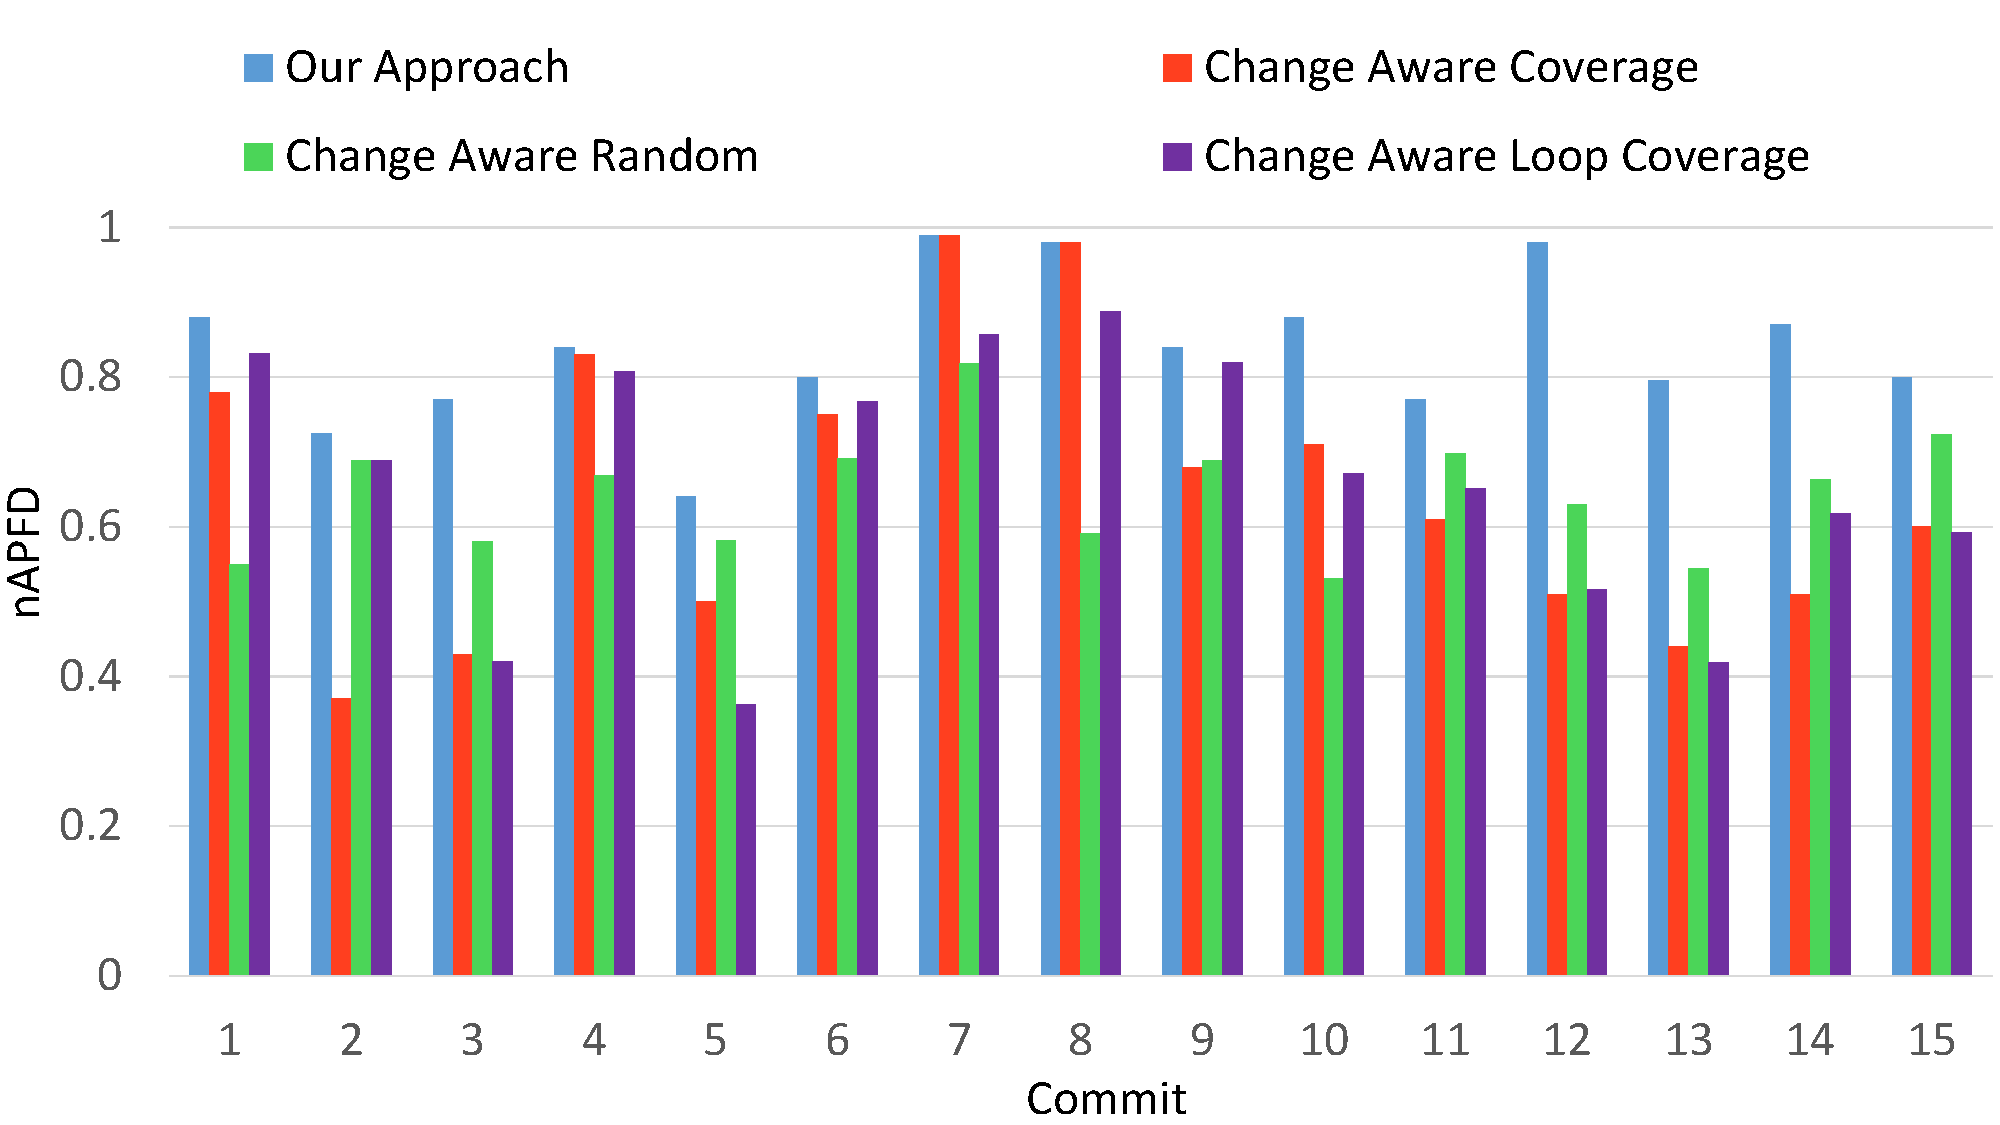
\includegraphics[width=4in, height=2.5in]{performance/images/common-math-apfd.pdf}
		
		\caption{\textit{APFD-P} Comparison on Apache Commons Math}	
		\label{fig:common-math-apfd}


\end{figure}

\begin{figure}
		\centering
		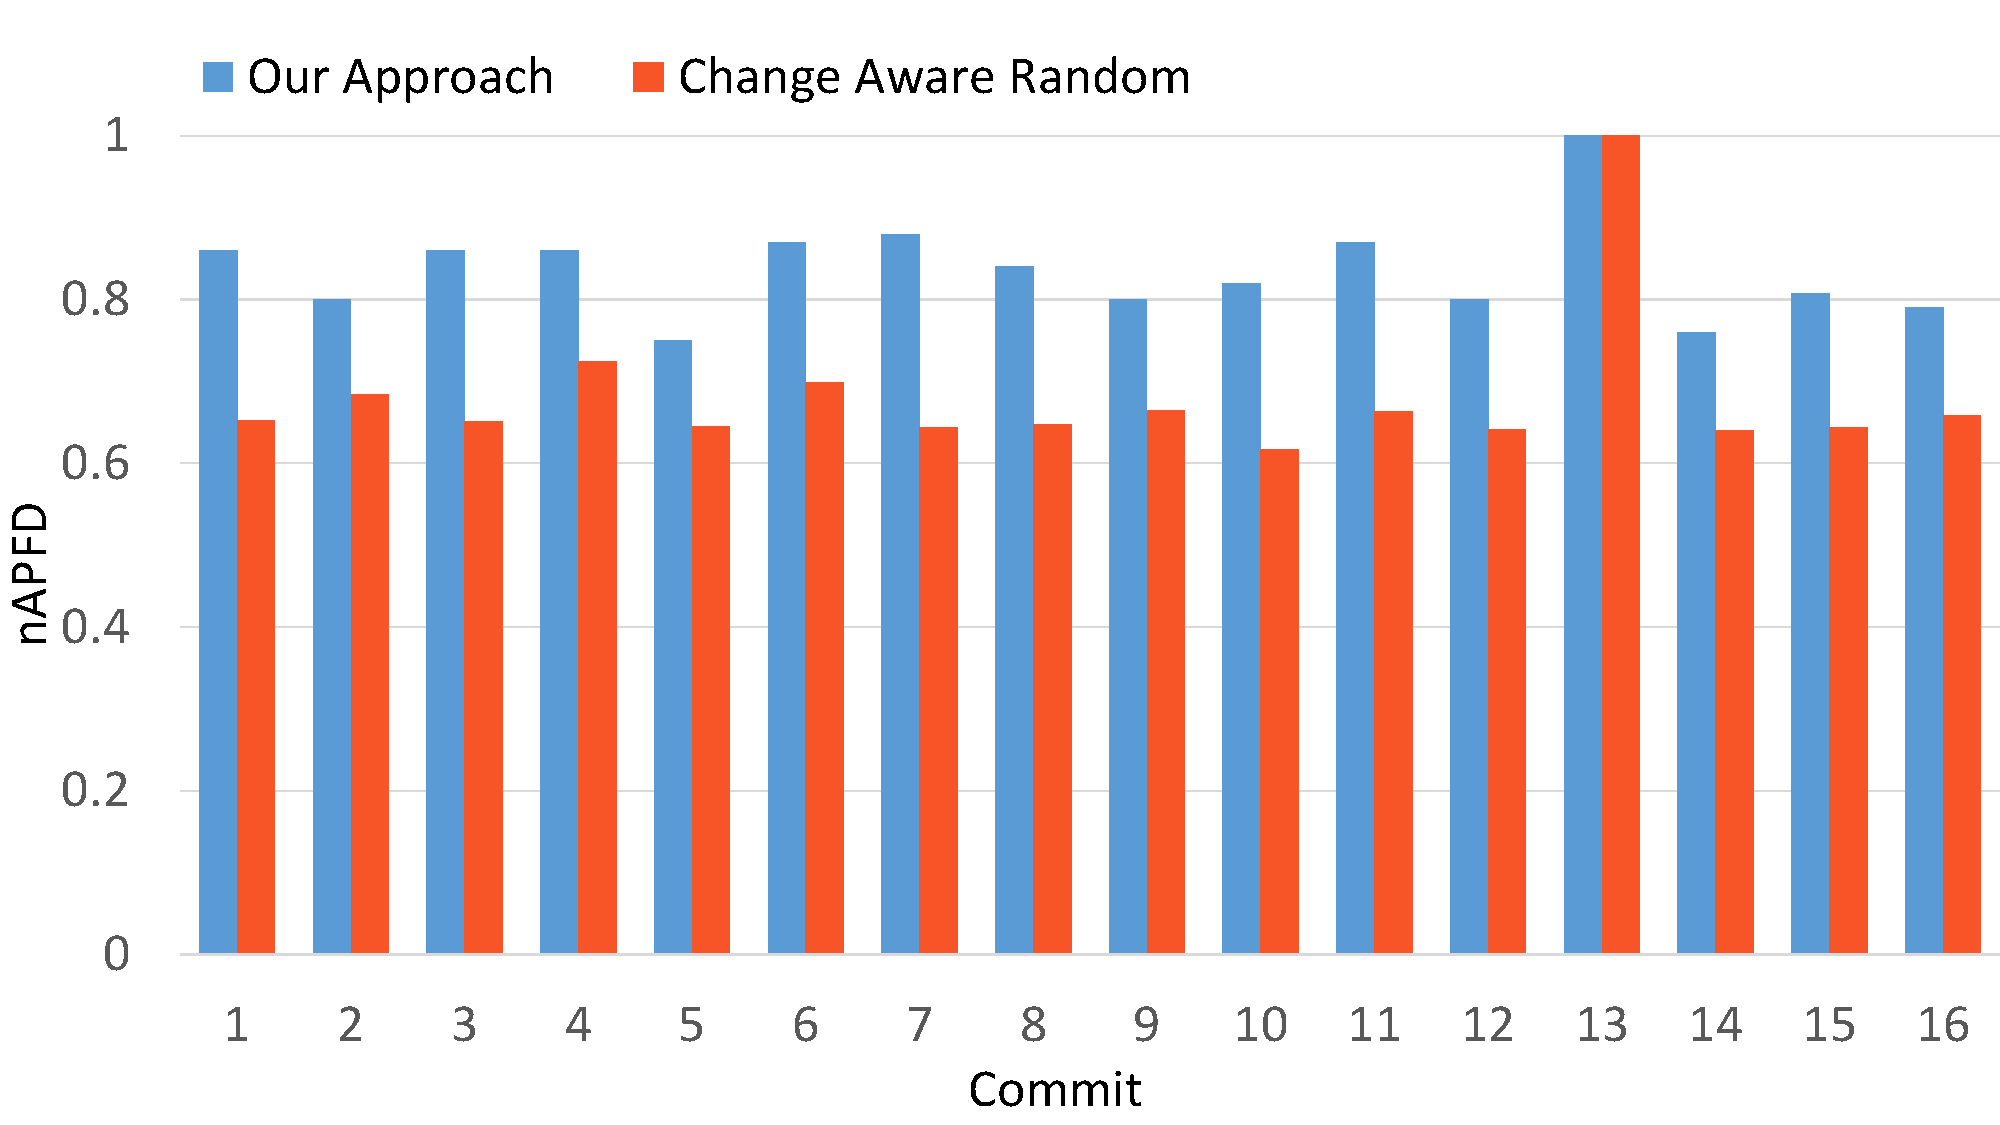
\includegraphics[width=4in, height=2.1in]{performance/images/xalan-apfd.pdf}
			
		\caption{\textit{APFD-P} Comparison on Xalan}
	
		\label{fig:xalan-apfd}
\end{figure}

%\begin{figure}
%		\centering
%		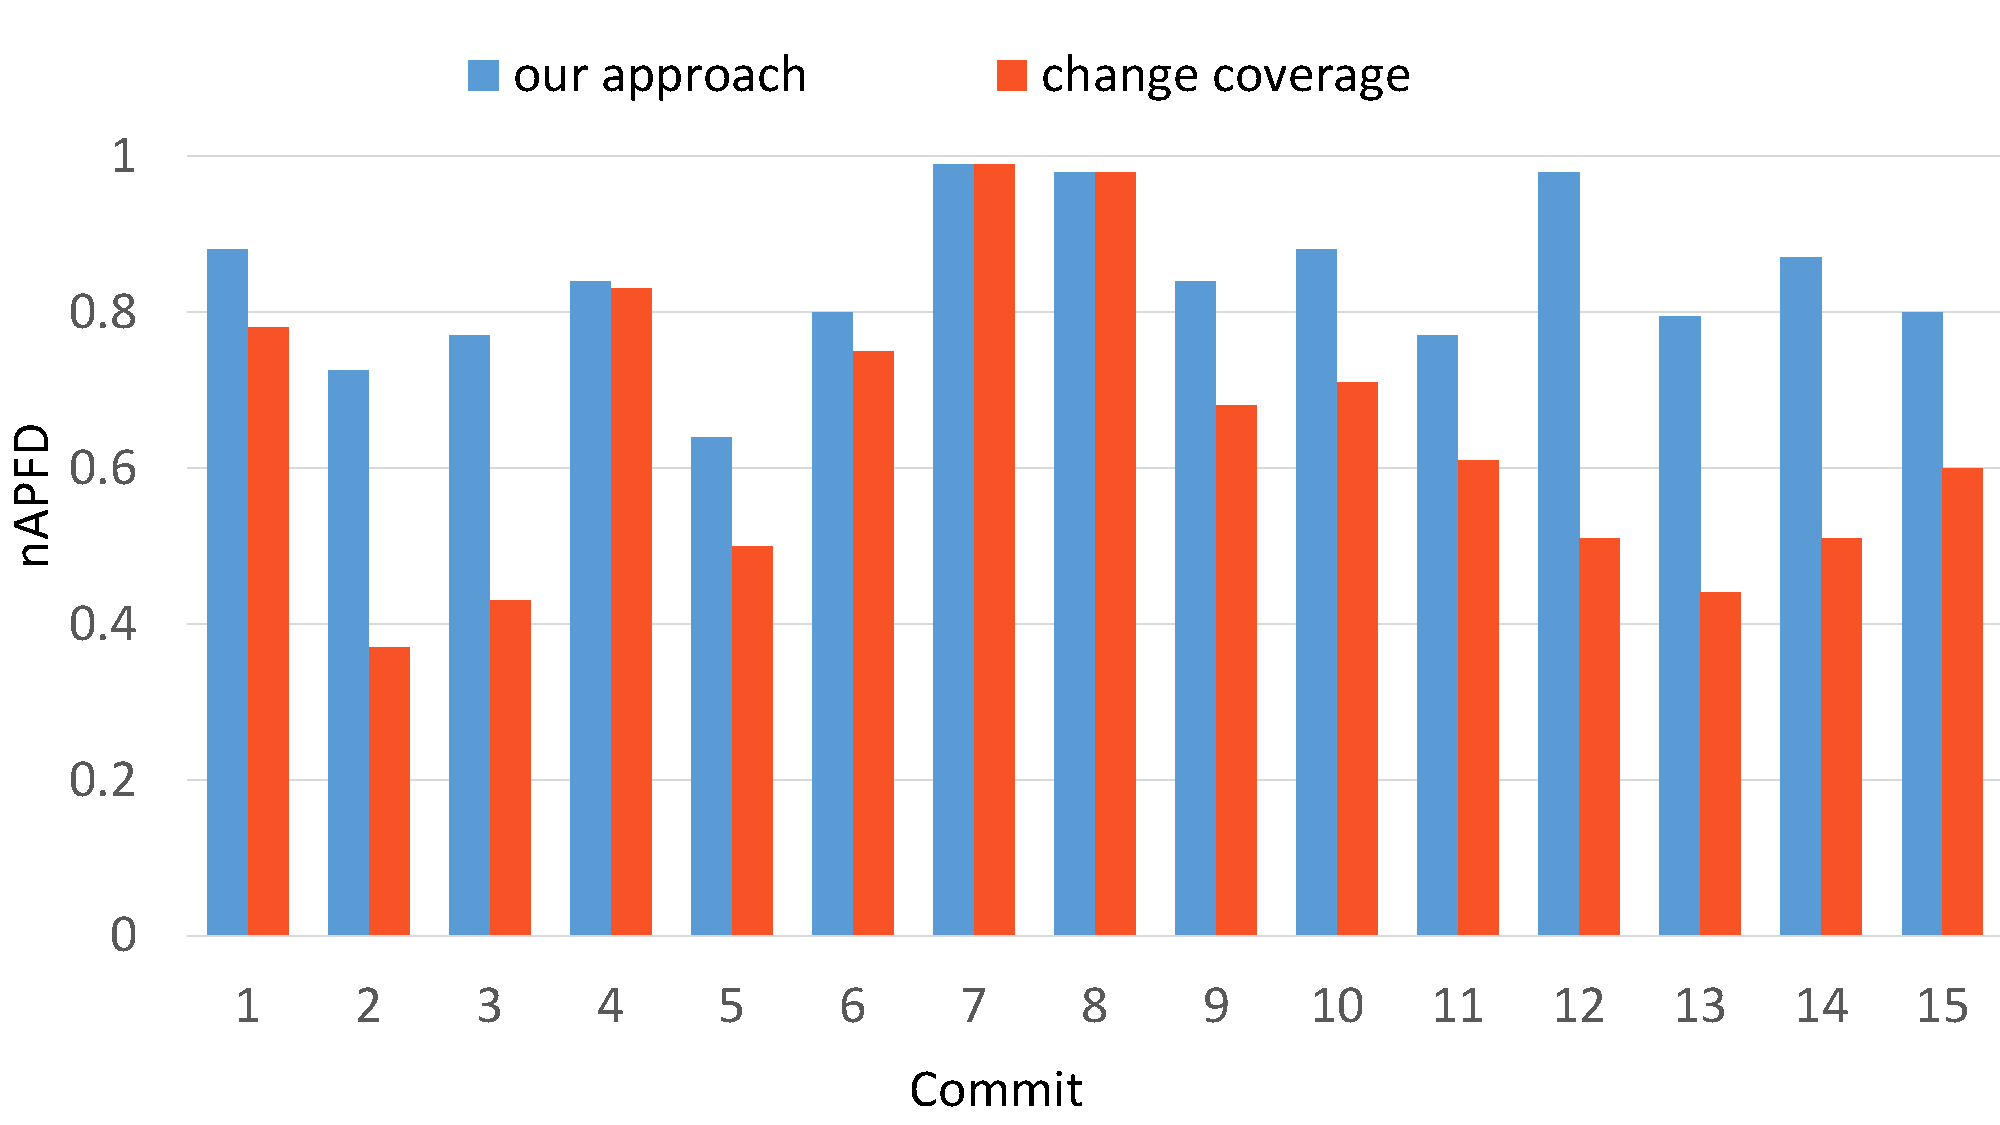
\includegraphics[width=\columnwidth]{images/common-math-coverage-apfd.pdf}
%		\caption{APFD-P Comparison with Change-Aware Coverage on Apache Commons Math}	
%		\label{fig:common-math-coverage-apfd}
%\end{figure}
%
%\begin{figure}
%		\centering
%		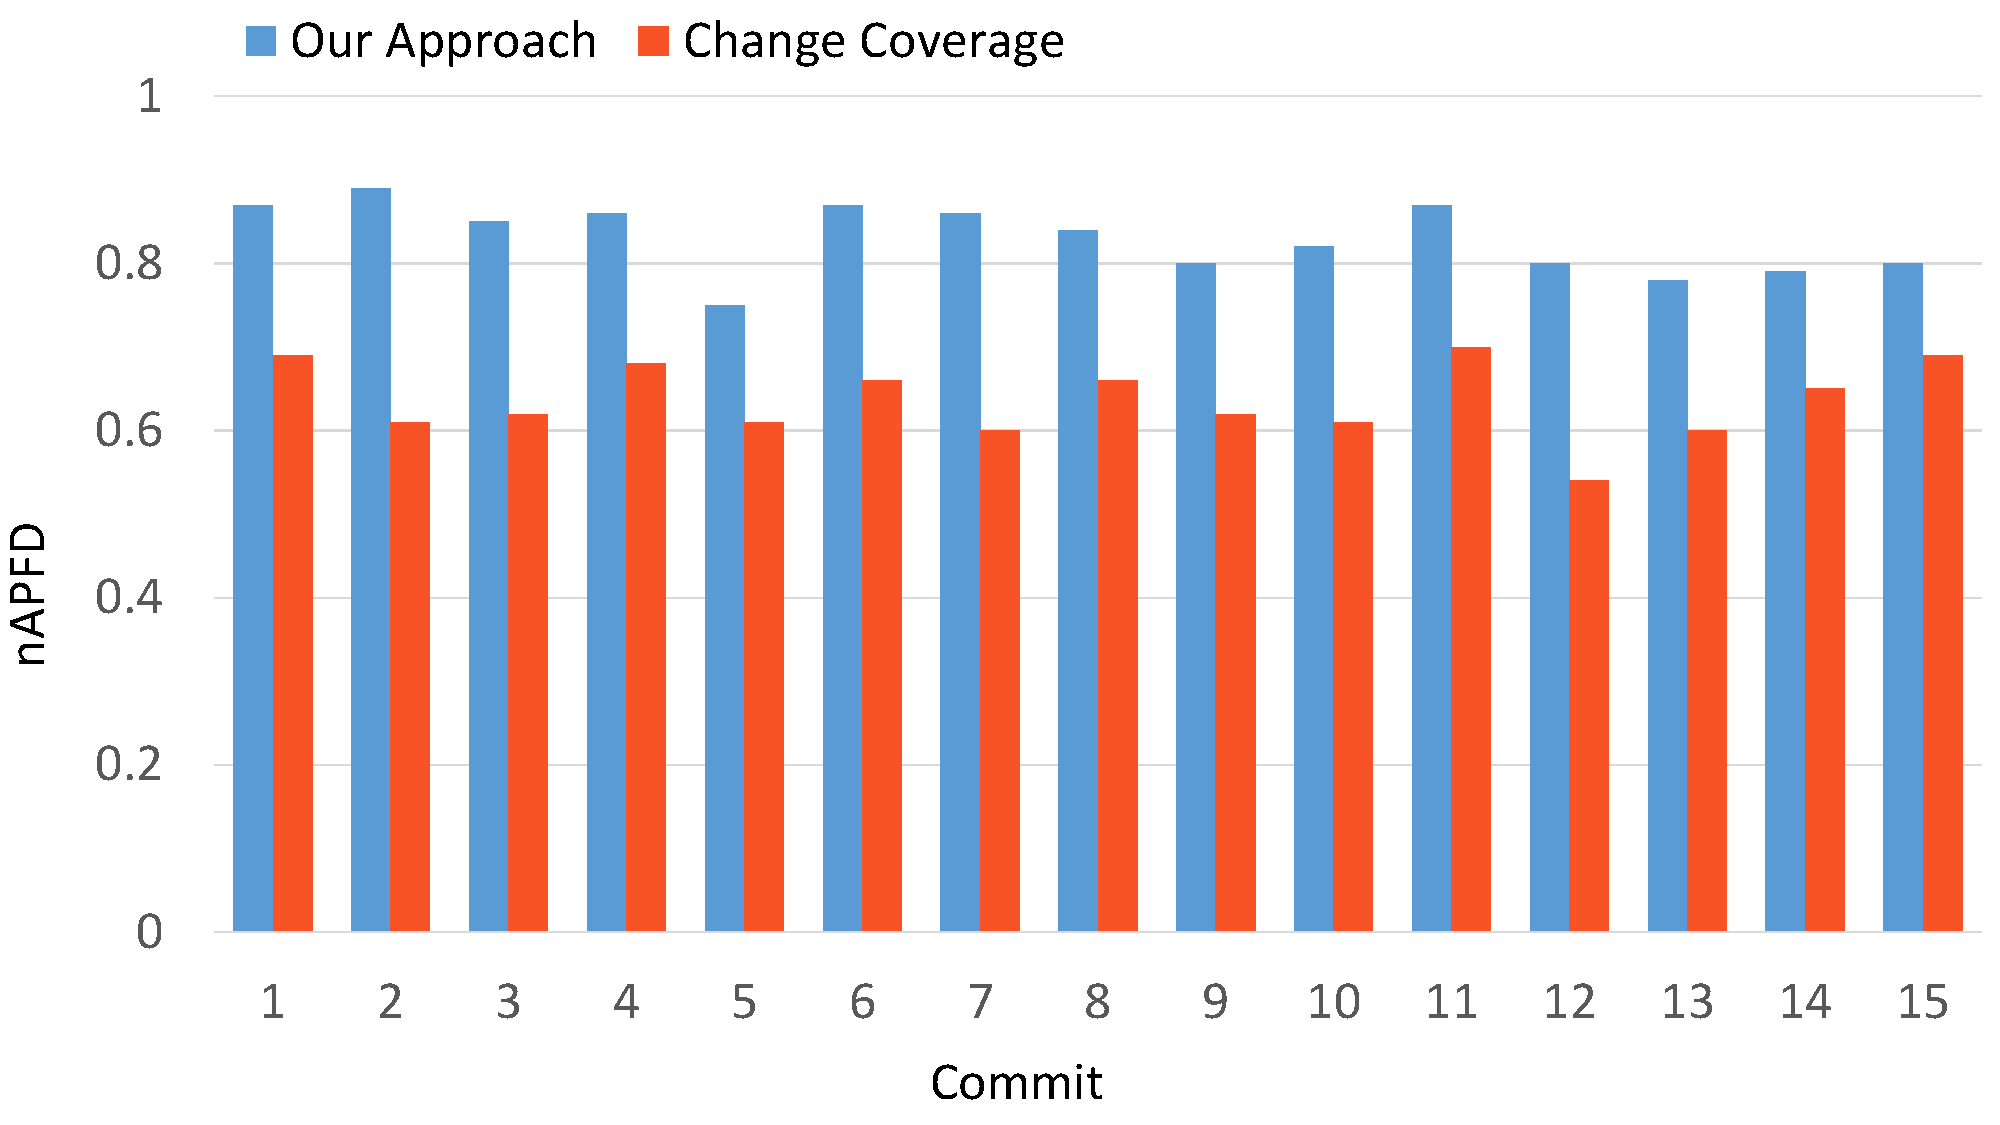
\includegraphics[width=\columnwidth]{images/xalan-coverage-apfd.pdf}
%		\caption{APFD-P Comparison with Change-Aware Random on Xalan}	
%		\label{fig:xalan-coverage-apfd}
%\end{figure}

Figures~\ref{fig:common-math-apfd} and~\ref{fig:xalan-apfd} show that our approach is able to achieve over 80\% \textit{APFD-P} value in most code commits affecting performance, and outperforms or rivals all baseline approaches in all code commits affecting performance from both subject projects. Specifically, for Apache Commons Math, our approach achieves an average \textit{APFD-P} value of 83.7\%, compared with 64.3\% by CAR, 64.6\% by CAC, and 66.1\% by CALC. For Xalan, our approach achieves an average \textit{APFD-P} value of 83.5\%, compared with 65.8\% by CAR, 63.6\% by CAC, and 59.8\% by CALC. Therefore, the improvement on the average \textit{APFD-P} is at least 17 percentage points, compared with baseline approaches on both projects. Furthermore, we do not observe significant effectiveness downgrade in the later versions, indicating that one base version can be used for a relatively long time.

%although we concede that the result may be due to the 

%Therefore, our approach is able to improve the APFD-P 


%In the figure \ref{fig:common-math-apfd}, we can see that overall nAPFD of our approach in Apache common math on the average 21.5\% greater than change aware random approach. In all the version our approach out perform random approach.





\subsubsection{\textit{nDCG} Metrics}

Similarly, Figures~\ref{fig:common-math-dcg} and~\ref{fig:xalan-dcg} show the comparison results between our approach and the three baseline approaches on the \textit{nDCG} metric. 

\begin{figure}
\centering
		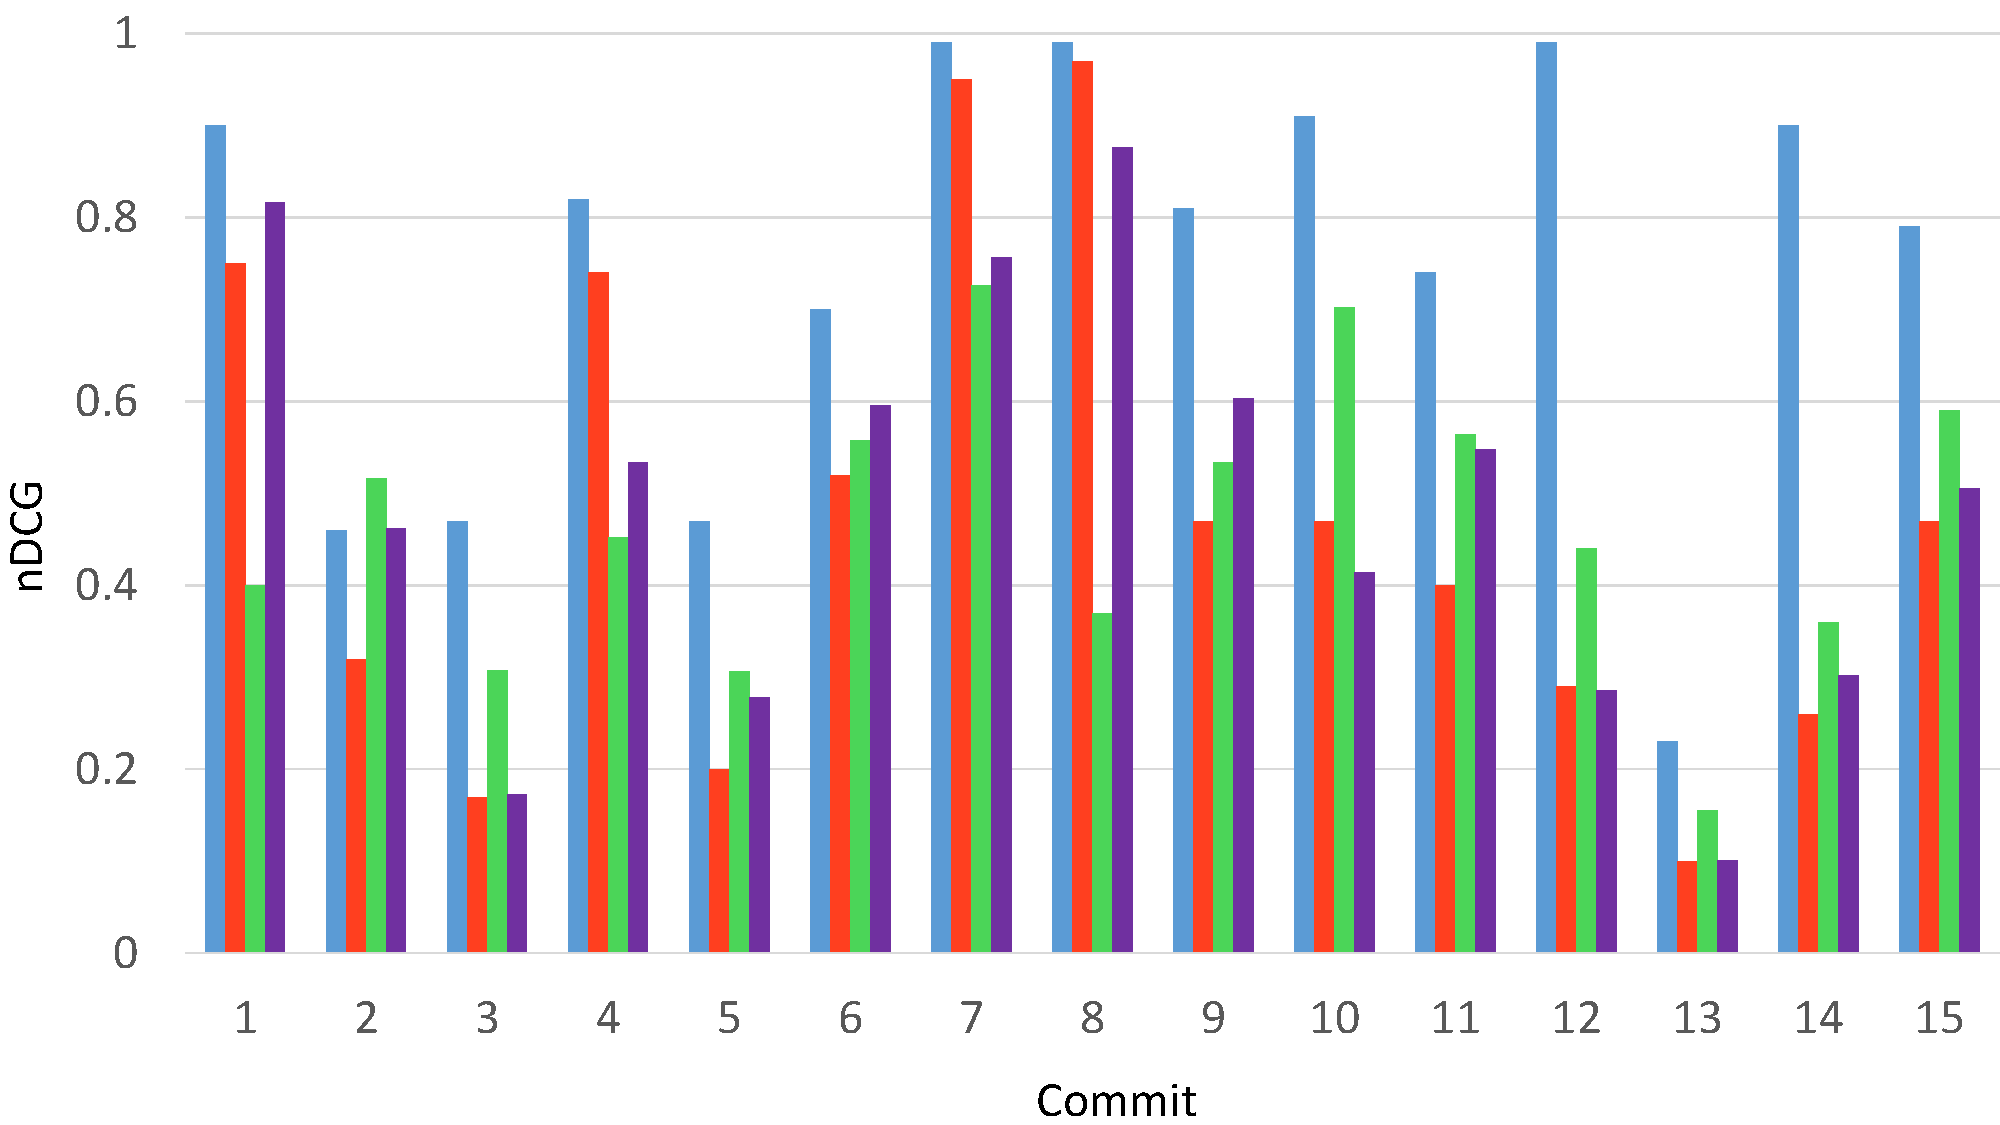
\includegraphics[width=4in, height=2.1in]{performance/images/common-math-dcg.pdf}
			
		\caption{\textit{nDCG} Comparison on Apache Commons Math}	
		\label{fig:common-math-dcg}
\end{figure}

\begin{figure}
\centering
		
		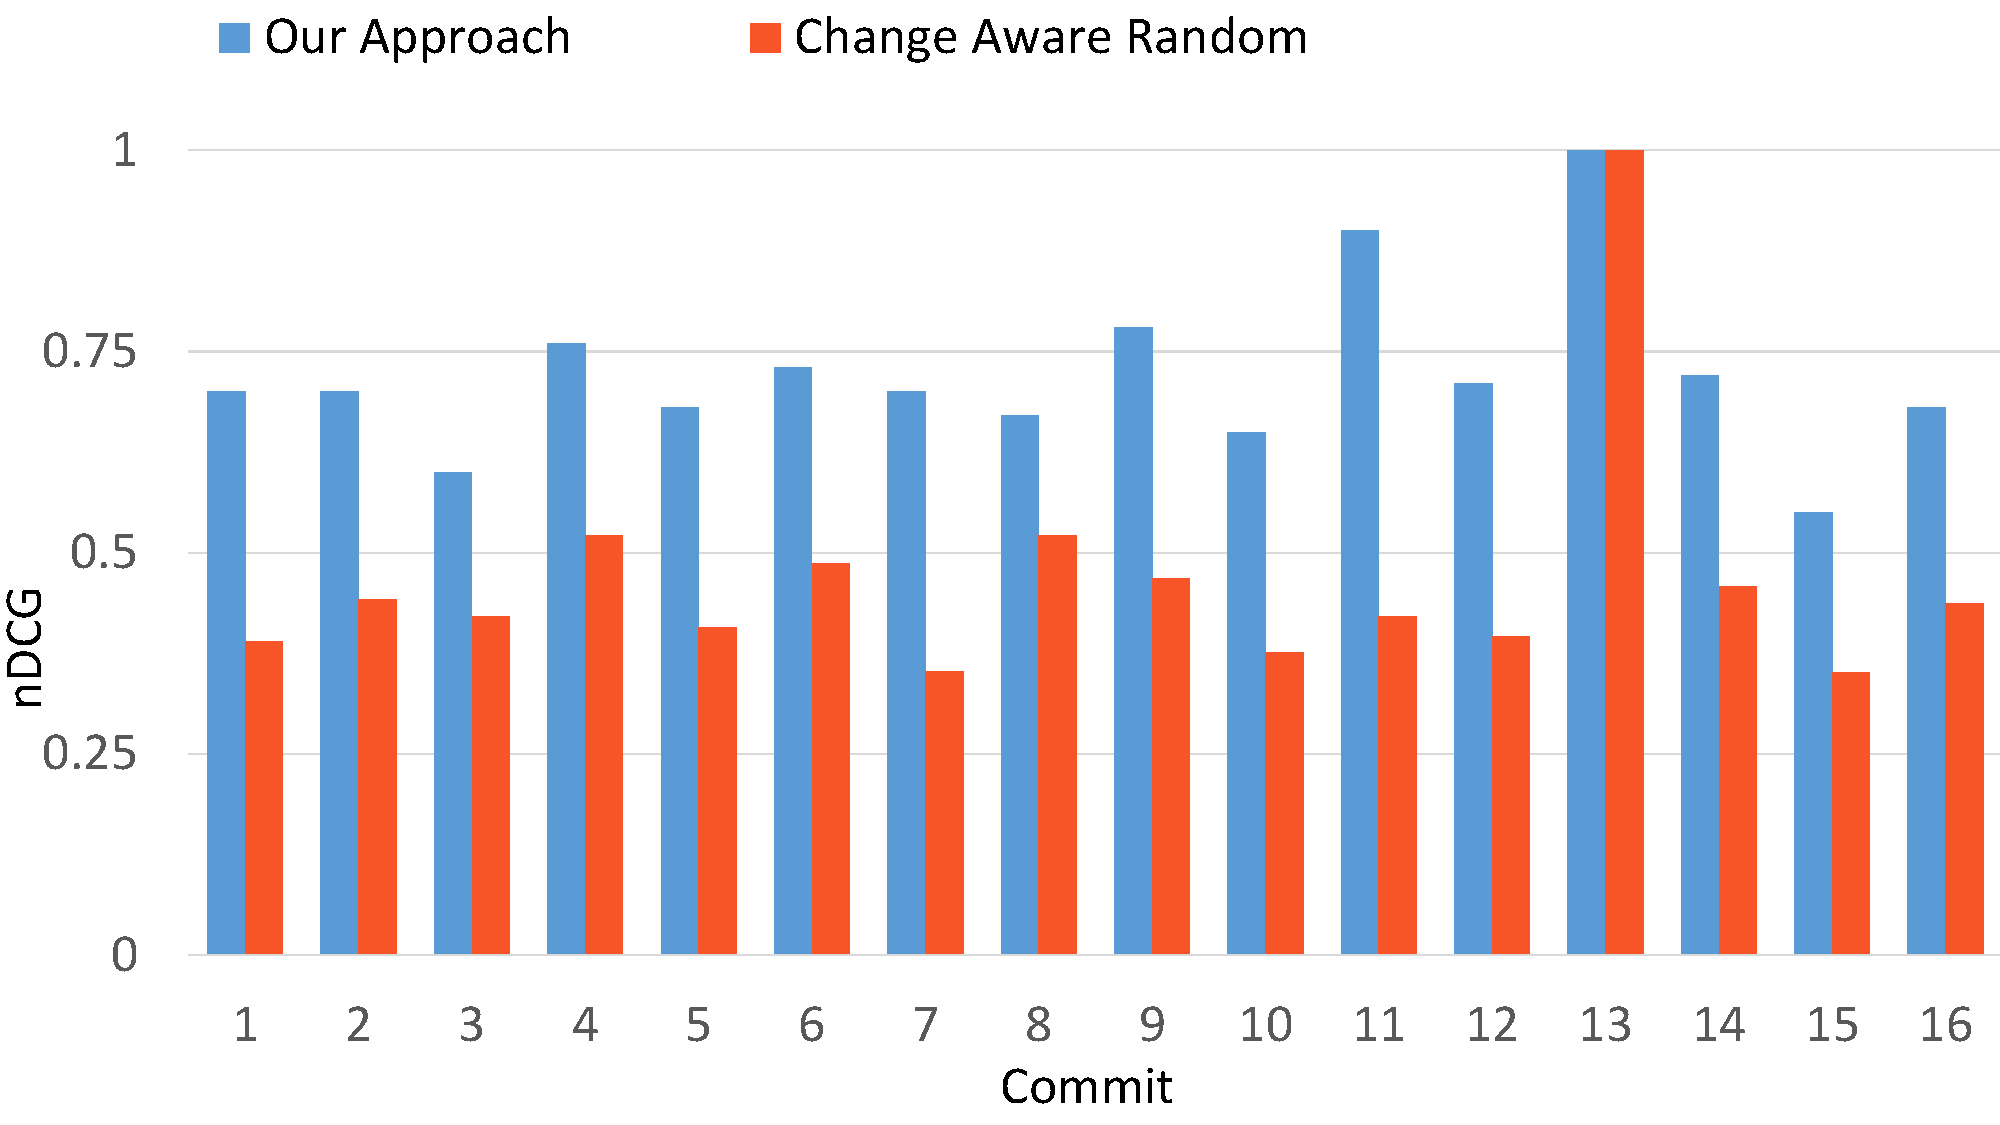
\includegraphics[width=4in, height=2.1in]{performance/images/xalan-dcg.pdf}
			
		\caption{\textit{nDCG} Comparison on Xalan}	
		\label{fig:xalan-dcg}
\end{figure}


%\begin{figure}
%		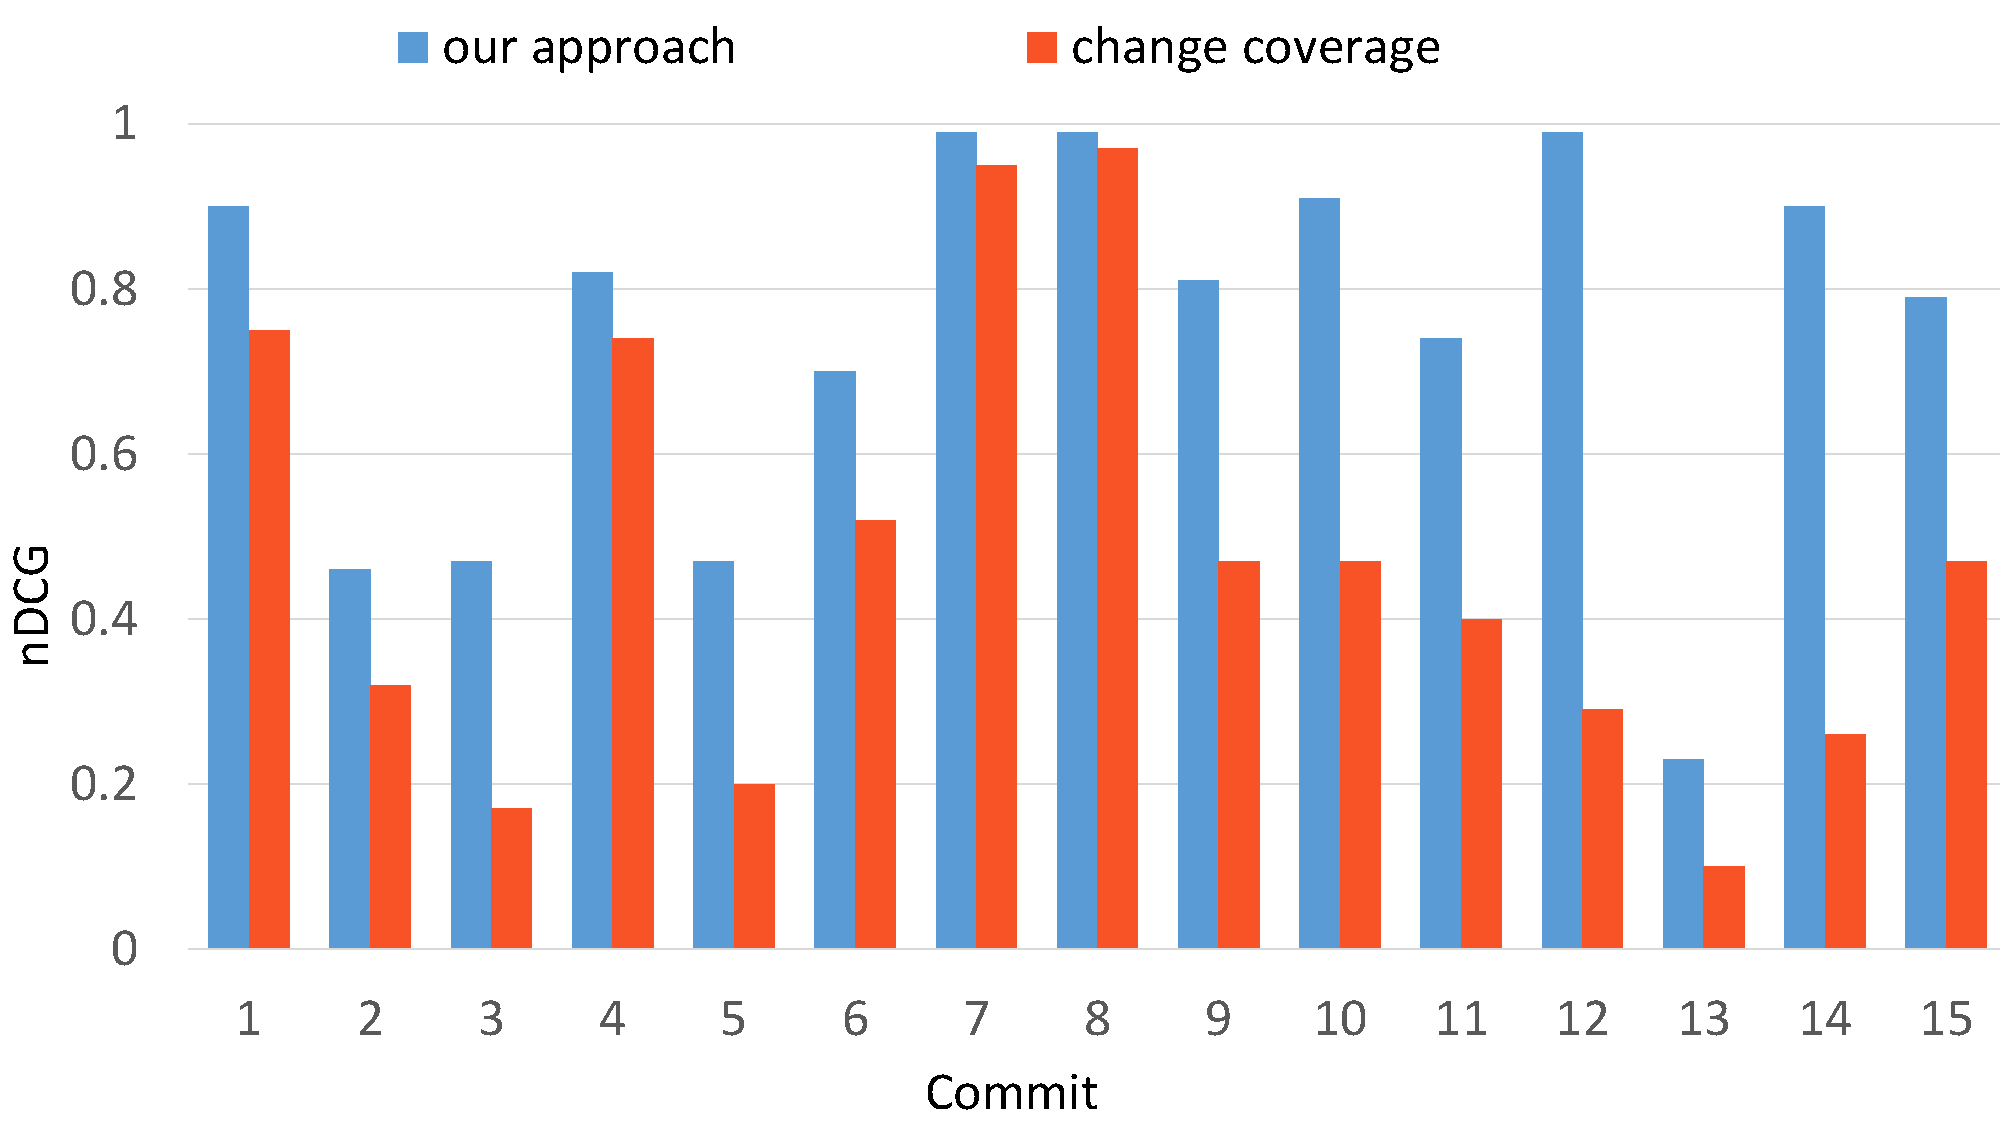
\includegraphics[width=\columnwidth]{images/common-math-coverage-dcg.pdf}
%		\caption{nDCG Comparison with Change-Aware Coverage on Apache Commons Math}	
%		\label{fig:common-math-coverage-dcg}
%\end{figure}
%
%\begin{figure}
%		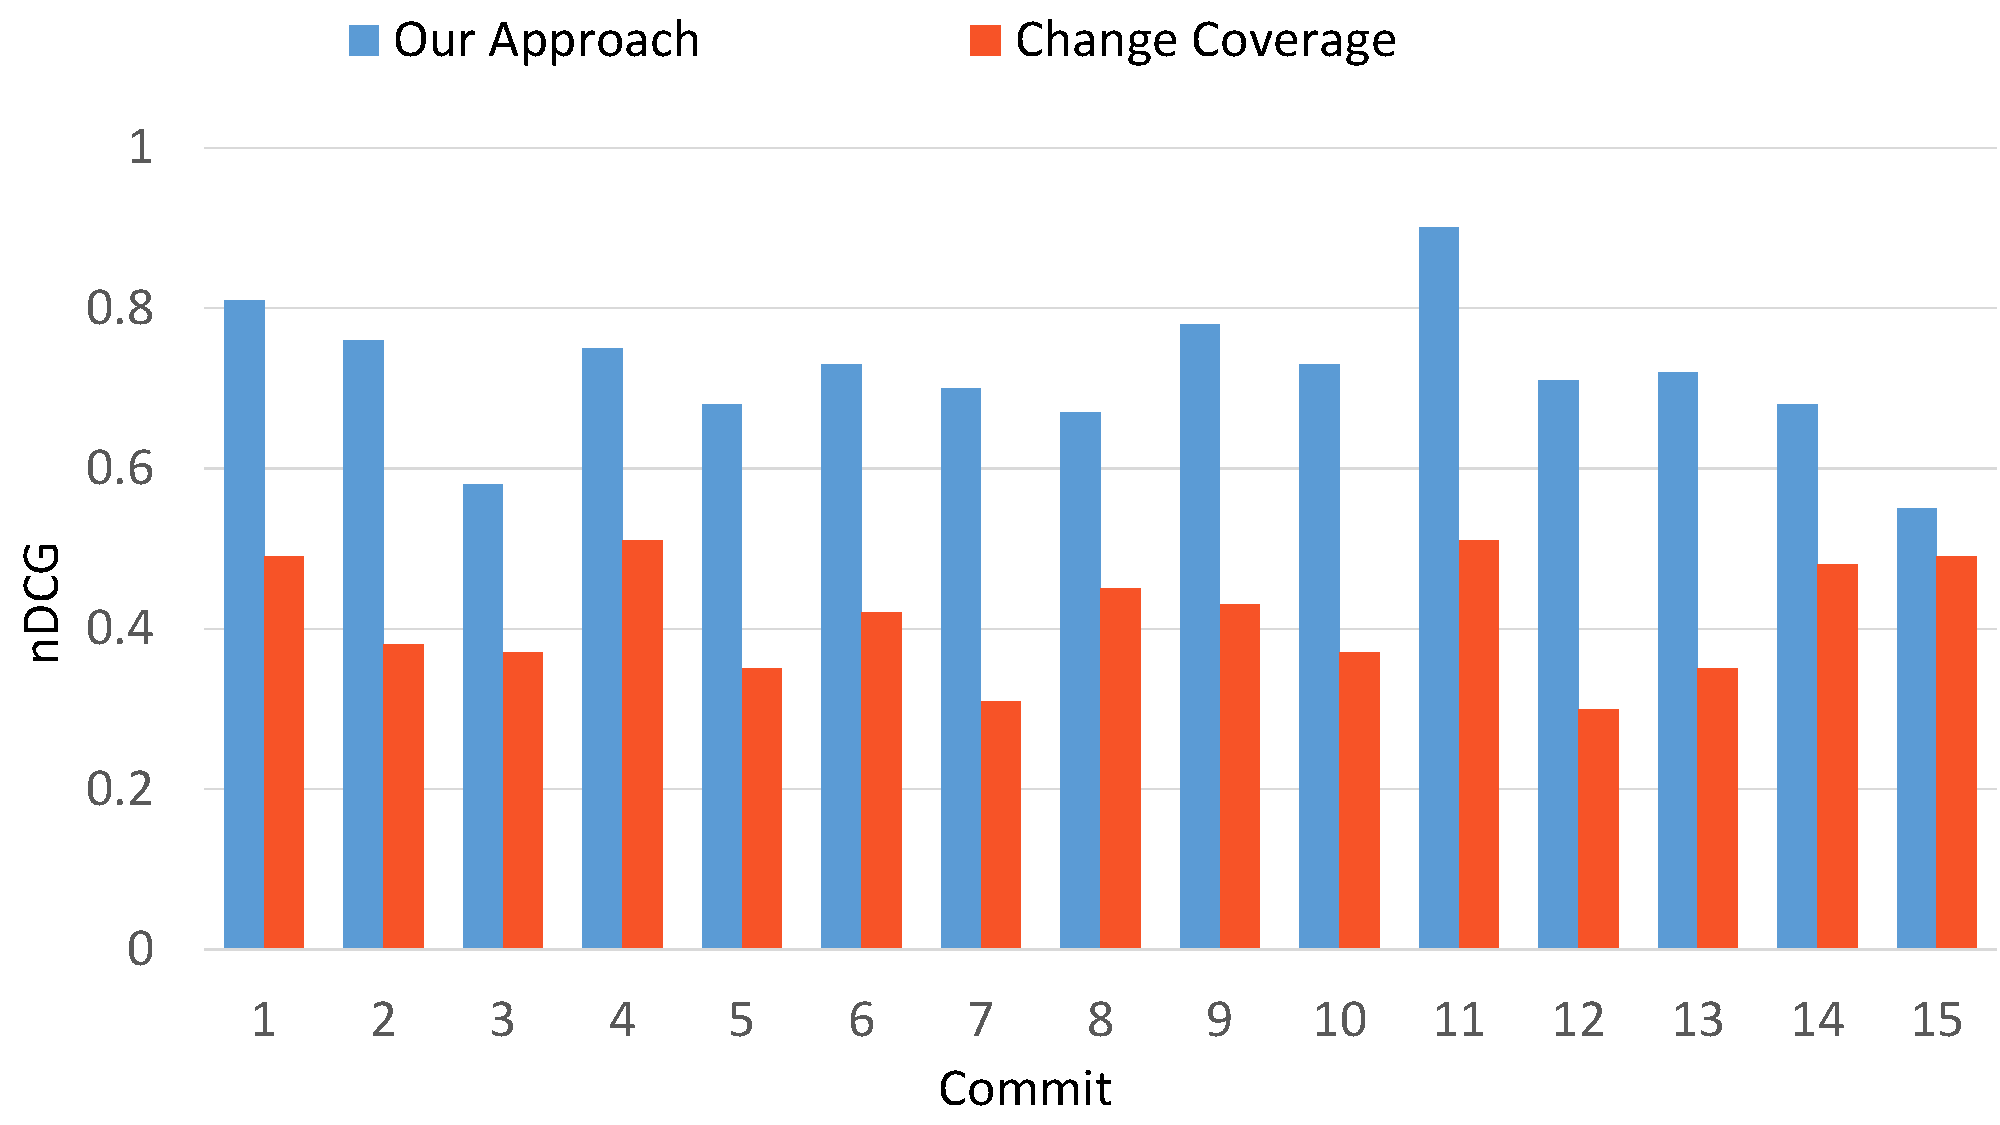
\includegraphics[width=\columnwidth]{images/xalan-coverage-dcg.pdf}
%		\caption{nDCG Comparison with Change-Aware Coverage on Xalan}	
%		\label{fig:xalan-coverage-dcg}
%\end{figure}

The figures show that our approach outperforms or rivals baseline approaches on \textit{nDCG} in almost all code commits from both subject projects. Specifically, for Apache Commons Math, our approach achieves an average \textit{nDCG} value of 74.5\%, compared with 47.2\% by CAR, 46.5\% by CAC, and 48.4\% by CALC. For Xalan, our approach achieves an average \textit{nDCG} value of 71.7\%, compared with 43.0\% by CAR, 41.4\% by CAC, and 37.4\% by CALC. Therefore, the improvement on the average \textit{nDCG} is over 26 percentage points on both projects. We also observe that there is one code commit from Xalan, in which our approach performs slightly worse than CAR on \textit{nDCG}. In Section~\ref{sec:qualitative}, we further discuss the details of this code commit in Listing~\ref{list:example-n1}.

Finally, we observe that compared with \textit{APFD-P}, the \textit{nDCG} values are generally lower and vary more significantly from code commit to code commit. The reason is that an \textit{nDCG} value is more sensitive to the rank of test cases with the highest performance impacts. For example, consider a test sequence with 100 test cases and only 1 test case has performance impact, and the performance impact value is 100\%. When this test case is ranked top, both \textit{APFD-P} and \textit{nDCG} are 1.0. However, if this test case is ranked $25^{th}$ in the sequence, the \textit{APFD-P} value is still as high as 75\%, but the \textit{nDCG} value becomes $1/log_2(25)$, which is less than 25\%. This result is reasonable because in information retrieval (where \textit{nDCG} was first  proposed), ranking the most relevant result at the $25^{th}$ position is very bad, but in test prioritization (where \textit{APFD} was first proposed), ranking the test case at the $25^{th}$ position is not so bad, because only 25\% test cases need to be executed to execute the test case. Therefore, which of \textit{APFD-P} and \textit{nDCG} is a better metric may depend on whether developers are interested in only a few most severely affected test cases, or a larger number of test cases whose performance is affected. 

%find that overall nDCG is higher comparison to nAPFD due to reason of penalising top impacted test case which are lower in the order. In some version improvement is much higher comparative to  


%The proposition of high nDCG is that highly relevant result appearing at the top. In the figure \ref{fig:common-math-dcg}, we can see that overall nDCG of our approach in Apache common math on the average 29.29\% greater than change aware random approach. 



%some other version for several reason is discussed above. Similarly, in the figure \ref{fig:xalan-dcg}, we can see that overall nDCG of our approach in Xalan on the average 27.21\% greater than change aware random approach.  \\
 


%We further compare our approach with change coverage approach. In figure \ref{fig:common-math-coverage-apfd}  and \ref{fig:xalan-coverage-apfd} shows the comparison of our approach with change coverage approach on  metric APFD. Our approach in common math on the average APFD score 0.85 whereas change coverage  average APFD score 0.68 (17\% greater). Similary, Our approach in xalan on the average APFD score 0.83 whereas change coverage  average APFD score 0.63 (19\% greater).In figure \ref{fig:common-math-coverage-dcg}  and \ref{fig:xalan-coverage-dcg} shows the comparison of our approach with change coverage approach on  metric DCG. Our approach in common math on the average DCG score 0.77 whereas change coverage  average DCG score 0.53 (24\% greater). Similary, Our approach in xalan on the average DCG score 0.71 whereas change coverage  average DCG score 0.41 (30\% greater).\\

\subsubsection{Top-N Percentile}

While \textit{APFD-P} and \textit{nDCG} are normalized quantitative metrics for our problem, they are not sufficiently intuitive for understanding the direct benefit of our approach on developers. Therefore, we further measure how many test cases developers need to consider if they want to cover the top 3 most affected test cases. Tables~\ref{tab:math} and~\ref{tab:xalan} show the results. Columns 1 and 2 present the code commit number and the total number of test cases affected by the code commit, respectively. Columns 3-6 and 7-10 present the top proportion of ranked test cases required to cover top 1 and 3 most-performance-affected test cases\footnote{The results for top 2 show similar trends and are available on the project website~\cite{perfranker}}. 

%In each column group, the first column presents our result, and the remaining columns present the results of CAC, CALC, and CAR, respectively. 

%In each cell, the number in the bracket shows the percentage of test cases need to be considered. 



\begin{table}
\scriptsize
	\centering
	\caption{Top-N Percentile of Apache Commons Math}
	\label{tab:math}	
	
	\begin{tabular}{r|r||r|r|r|r||r|r|r|r}
	\hline
C &T & \multicolumn{4}{c||}{Top 1} & \multicolumn{4}{c}{Top 3} 
\\  \cline{3-10}
\#  & \#   & Our & CAC & CALC & CAR &  Our & CAC & CALC & CAR\\\hline
	1 & 55 & 2\% & 3\%& \textbf{1\%} & 49\% & \textbf{6\%} & 43 & 27\%& 74\%\\
	2 & 60     & 40\%& 61\%& \textbf{38\%} & 49\% & \textbf{51\%} & 61\% & 93\% & 74\%\\
	3 & 152     & \textbf{2\%} & 84\%& 79\%& 49\%  & \textbf{28\%} & 88\% & 88\% & 74\% \\
	4 & 97      & \textbf{3\%} & 18\%& 87\% &  49\%  & \textbf{5\%} & 18\% & 87\% & 74\% \\
	5 & 130    & \textbf{4\%} & 29\% & 43\% & 49\% & \textbf{4\%} & 96\% & 97\% & 74\%  \\
	6 & 15     & \textbf{13\%} & 40\%& 33\%&46\% & 66\% & \textbf{40\%} & 100\% &  73\% \\
	7 & 18      & \textbf{5\%} & \textbf{5\%} & 88\% & 47\% & \textbf{15\%} & 40\% & 88\% & 74\%\\
	8 & 10     & \textbf{10\%} & \textbf{10\%} & 40\% &45\%  & \textbf{60\%} & \textbf{60\%} & 70\%& 70\%\\
	9 & 12     & \textbf{8\%} & 66\%&75\% & 45\% & \textbf{50\%} &66\% & 75\%& 72\%\\
	10 & 12      & \textbf{8\%} & 50\% & 83\% & 45\% & 83\% & \textbf{50\%} & 100\% & 72\% \\
	11 & 36      & \textbf{5\%} & 94\%& 38\% & 48\% & 66\% & 94\%& \textbf{58\%} & 74\%\\
	12 & 13     & \textbf{7\%} & 76\% & 38\%& 45\% & 76\% & 84\%& 100\%& \textbf{72\%} \\
	
	13 & 711    & \textbf{7\%} & 81\%& 84\% & 49\% & \textbf{7\%} & 81\%& 84\%& 74\% \\
	14 & 39      & \textbf{2\%} & 84\%& 25\%& 48\% & \textbf{12\%} & 84\% & 79\% & 74\% \\
	15 & 34      & \textbf{11\%} & 52\% & 17\% & 48\% & \textbf{26\%} & 58\%& \textbf{26\%} & 74\%\\ \hline
	Avg      &   & \textbf{8\%} & 50\% & 51\% & 48\%  & \textbf{37\%} & 65\% & 78\% & 73\% \\  \hline
	\end{tabular}
\end{table} 

\begin{table}
\centering 
\caption{Top-N Percentile of Xalan}
	
\label{tab:xalan}
\scriptsize
\begin{tabular}{r|r||r|r|r|r||r|r|r|r}
\hline
C &T & \multicolumn{4}{c||}{Top 1} & \multicolumn{4}{c}{Top 3} 
\\  \cline{3-10}
\#  & \#   & Our & CAC  & CALC & CAR&  Our  & CAC  & CALC & CAR\\\hline
1 & 63     & 20\%& 46\% & \textbf{14\%} & 49\% & \textbf{36\%} & 60\% & 50\% & 74\% \\
2 & 63   & \textbf{17\%} & 85\% & 22\% & 49\%& \textbf{17\%} & 85\%& 80\%&74\% \\
3 & 63      & \textbf{7\%} & 85\% & 50\% & 49\%  & \textbf{38\%} & 85\% & 66\% & 74\% \\
4 & 63   &  20\%& 80\% & \textbf{7\%} & 49\% & \textbf{20\%} & 85\% & 73\% & 74\% \\
5 & 63   & \textbf{6\%} & 85\% &  100\% & 49\% & \textbf{53\%}  & 85\% & 100\% & 74\%\\
6 & 63      & \textbf{11\%} & 63\% & 31\% & 49\% & \textbf{26\%} & 76\% & 77\% & 74\% \\
7 & 63   & \textbf{11\%} & 46\% &  12\% & 49\% & \textbf{15\%} & 85\% & 93\% & 74\% \\
8 & 63    & \textbf{9\%}  & 35\% & 36\% & 49\% & \textbf{20\%} & 82\% & 95\% & 74\% \\
9 & 58      & \textbf{3\%} & 96\% &  5\% & 49\% & \textbf{25\%} & 96\% & 98\% & 74\% \\
10 & 63   & 30\% & 47\% & \textbf{17\%} & 49\% & \textbf{31\%} & 85\% & 84\% & 74\% \\
11 & 63   & \textbf{1\%} & 31\% & 12\% & 49\% &  \textbf{7\%}  & 62\% & 74\% & 74\% \\
12 & 63     & \textbf{23\%} & 85\% & 88\% & 49\% & \textbf{34\%} & 90\% & 88\% & 74\%\\
13 & 63     & \textbf{12\%} & 46\%& 82\% & 49\%  & \textbf{53\%}  & 65\%& 82\% &74\% \\
14 & 58    & 34\% & 34\% & \textbf{8\%} & 49\% & 43\% & \textbf{37\%}  & 72\% & 74\% \\ 
15 & 63     & 36\% & \textbf{4\%} & 12\% & 49\% & \textbf{36\%} & 79\%& 61\% & 74\% \\ \hline
Avg        & & \textbf{16\%} & 57\%  & 34\% & 49\%& \textbf{30\%} & 77\%  & 79\% & 74\% \\		\hline
\end{tabular}
\end{table}

%For example, change version-3 touches 13 test case and actual impact score of top test case 1st,2nd and 3rd are 0.75, 0.07 and 0.06 respectively. Our approach ranked them with impact score 7.57,2.36 and 2.35 where overall nAPFD score of approach is 0.98 compared to change aware random score 0.63 that is 35\% improvement.


%Performance regression testing cost reduction is highly desirable. For example, running few top impacted test case can save a lot of testing time. Keep that goal in mind, we evaluated our result and We consider only those changes that touches more than three test case in the table \ref{tab:math} and \ref{tab:xalan}. 

Tables~\ref{tab:math} and~\ref{tab:xalan} show that on average our approach is able to cover Top 1 and 3 most-performance-affected test cases within top 8\%, 21\%, and 37\% of ranked test cases in Apache Commons Math, and 16\%, 22\%, and 30\% of test cases in Xalan. The improvements over the baselines approaches are at least 33\%, 37\%, and 28\%. Furthermore, on top 1 coverage, our approach outperforms or rivals the best baseline approach on 13 code commits from Apache Commons Math, and 10 code commits from Xalan. On top 3 coverage, our approach achieves the highest percentage on 11 code commits from Apache Commons Math, and 14 code commits from Xalan. 

%Also, our approach generates better result for Top 1 for code commits affecting fewer test cases, but better result for Top 3 for code commits affecting more test cases. The major reason is that, for code commit affecting fewer test cases, maybe only 1 or 2 test cases are affected with high performance impact. So the 3rd most affected test case may be not very different from other test cases. Actually, one drawback of using Top N coverage as metrics is that, it does not taking into account the actual performance impact, which is considered in $APFD-P$ and $nDCG$.


%consistently better than the two baseline approaches on most code commits, and 


\subsubsection{Overhead and Performance}
In test prioritization, it is important to make sure that the time spent on prioritization is much smaller than the execution time of performance test cases. To confirm indeed that is the case, we record the overhead and execution time of our analysis. Our profiling of the base version has a 1.92 times overhead on Apache Commons Math, and 5.18 times overhead on Xalan. The static analysis per test case takes 29.90 seconds on Apache Commons Maths, and 34.35 seconds on Xalan. Finally, for Apache Commons Math, the average, minimal, and maximal time for analyzing a code commit are 45.35 seconds, 4.23 seconds, and 262.30 seconds, respectively, while for Xalan, the average, minimal, and maximal time for analyzing a code commit are 9 seconds, 3.36 seconds, and 21.80 seconds, respectively. In contrast, it takes averagely 52 (3) minutes to execute test suite of Apache Commons Math (Xalan) for 173 (47) times to achieve an expectation of equal to or less than 10\% execution-time variance.


%we can see that, top1 contains on the average within 8\% in common math and 16\% in xalan. That means more than 85\% test cases can be eliminated. Similarly top2 and top3 contain on the average within  21\% and 37\% respectively in common math and   22\% and 30\% respectively in common xalan. So on the average our approach eliminate 70\% test case to select top 3 impacted test case.


%These table show the result of Top1, Top2 and Top3 impacted test case position in the ranking order and contain within percentage result of apache common math and xalan. For example, first row in the table \ref{tab:math} represents that the changes in version-1 impacted test case 1st, 2nd and 3rd position in the ranked list is 11th,1st and 2nd respectively and top 3 impacted test case contain within 17\% in the ranked list. The changes in version-9 touches 55 test cases and their relative ordering perfectly match the actual ordering of top 3. The main reason is that relative impact difference between the test case distinguishable which means that 1st relative impact 3 to 5 times compared to 2nd and 3rd in this case. But the change on version-13 touches 711 test cases and the impact on test case are very similar and little difference in their relative order which is top1's relative impact score 1.05 to 1.13 times compared to 2nd and 3rd. Within 0.54 score interval contains 653 test case. So we can say that a good separation margin in performance impact among the order test case provide better ranking order. Though their position in the ranking above 50, top 3 contains within 7\%. 


%There is another commit version where our approach perform better than random but it is below 25\% compared to ideal. It is interesting that top 3 contain within 7\% in the ranked list which means it can eliminate 93\% test case. The reason of this issue is explained in later paragraph under Top percentage result evaluation. 



%\subsubsection{Summary of Findings}
%To sum up, our quantitative analysis has the following major findings. 

%\begin{itemize}
%	\item Our technique outperforms both 
%	\item 
%\end{itemize}


\subsection{Successful and Challenging Examples}
\label{sec:qualitative}
%In all the version our approach out perform random approach except one version which touches 60 test case and interestingly top 3 contain within 51\%. Though our approach is below random in this case, it can eliminate 60\% test case to select top impacted test case. The overall ranking does not perform well in this change because of the reason that conditional return or throws statement  added in the top of method body is shown in the listing\ref{fig:example-2}. As a result some of test case skip the whole execution of method which spend time inside loop in the method body in earlier version. 

In this section, with representative examples of code commits, we explain why our approach performs well on some code commits but not so well on some others. 

%Due to space limit, for each code commit, we present only the relevant changes instead of the whole commit. More details about our code commit examples can be found on our project website~\cite{perfranker}.

\textbf{Successful Example 1.} Listing~\ref{list:example-p1} shows the simplified code change of code commit hash d074054... of Xalan. On this code commit, our approach is able to improve the \textit{APFD-P} and \textit{nDCG} values by at least 13.53 and 31.22, respectively, compared with the three baseline approaches. In this example, several statements are added inside a loop. Our approach can accurately estimate the performance change because (1) Line 2 in the code is an existing loop and from the profile database for the base version we can find out exactly how many times it is executed, and (2) the added method invocations are combinations of existing method invocations whose execution time is already recorded for the base version. \\

%Combining the information in our performance model, we can precisely predict the performance impact of the change for each test case.


{\fontsize{10}{10}
\begin{lstlisting}[columns=flexible,language=Java,caption=Change Inside a Loop, label={list:example-p1}]
  int nAttrs = m_avts.size();
  for (int i = (nAttrs - 1); i >= 0; i--){
    ...
+   AVT avt = (AVT) m_avts.get(i);
+   avt.fixupVariables(vnames, cstate.getGlobalsSize());
    ...
  } 
\end{lstlisting}
}


\textbf{Successful Example 2.} Listing~\ref{list:example-p2} shows the simplified code change of code commit hash 64ec535... of Xalan. On this code commit, our approach is able to improve the \textit{APFD-P} and \textit{nDCG} values by at least 17.14 and 24.33, respectively, compared with the baseline approaches. In this example, the loop at Line 4 depends on the collection variable \CodeIn{m\_prefixMappings} at Line 1 whose size can be inferred from the recorded number of iterations of existing loops. In this case, our approach can accurately estimate the iteration count of this new loop and estimate the overall performance impact based on the estimated iteration count.\\

{\fontsize{10}{10}
	\begin{lstlisting}[columns=flexible,language=Java,caption=A Newly Added Loop Correlating to an Existing Collection, label={list:example-p2}]
	+ int nDecls = m_prefixMappings.size();
	+      
	+ for (int i = 0; i < nDecls; i += 2){
	+   prefix = (String) m_prefixMappings.elementAt(i);
	+   ...
	+ }     
	\end{lstlisting}
}

%Our approach can easily identity hot path and changes that lie in the hot path from our performance model which is constructed on the call graph. Beside these any intra procedure change that related to loop can estimate impact cost except few cases. But we believe that actual improvement is more than this score because running the regression with top impacted test case is enough for exposing performance problem and the probability of selecting top impacted test case 7\% in random. 

%Collection are generally propagated through function parameter and field variable. In Listing~\ref{list:example-p3}, at line 1 introduce new array list and at line 6 this list is updated under a existing loop. We can easily estimate the length of new array list. New method introduce that is not shown here that iterate of over the new list, our technique can predict the iteration of that loop. 

%{\fontsize{7}{7}
%\begin{lstlisting}[language=Java,caption=Collection Propagation, label={list:example-5}]
%+ Collections.sort(limits);

%+ for (int i = 0; i < limits.size(); i += 2) {
%  +list.add(new Arc(limits.get(i), limits.get(i + 1)));
%+}
%\end{lstlisting}
%}

%{\fontsize{7}{7}
%	\begin{lstlisting}[language=Java,caption=Correlation New and Existing Collection, label={list:example-p3}]
%	+ List processedDefs = new ArrayList();
%	
%	for (int i = 0; i < nAttrs; i++){
%	+
%	
%	+ processedDefs.add(attrDef);
%	+
%	
%	}
%	\end{lstlisting}
%}

%\textbf{Positive Example 3.} The simplified code change of code commit of Apache common math is presented in Listing~\ref{list:example-p3}. On this code commit, our approach is able to enhance $APFD-P$ and $nDCG$ by at least 34.12, and 48.35, compared with 3 baseline approaches but it is not presented in $APFD-P$ and $nDCG$ graph because the number of test cases affected by the change are less than 10. In Listing~\ref{list:example-p3}, at Lines 3-5, elements from the collection variable \CodeIn{limits} are added to another collection variable \CodeIn{list}. In this case, our collection propagation technique is able to link the two collection variables, and propagate the impact to the loops depending on variable \CodeIn{list}. It should be noted that, the iteration number of the loop is actually half of the size of \CodeIn{limits}. In our approach, for simplicity, we ignore different operations on the index variables and simply deem the loop-iteration numbers to be the same as the size of collections it depends on. Since test prioritization does not require exact prediction of performance impact, we found our approach to be still effective with such approximations (e.g., in this example). 
%
%{\fontsize{7}{7}
%\begin{lstlisting}[language=Java,caption=Collection Propagation, label={list:example-p3}]
%+final List<Arc> list = new ArrayList<Arc>();
%+ Collections.sort(limits);
% + for (int i = 0; i < limits.size(); i += 2) {
%  +list.add(new Arc(limits.get(i), limits.get(i + 1)));
%+}
%\end{lstlisting}
%}
%
%Although our approach is almost consistently better than the two baseline approaches and the improvement is significant, we still want to investigate the cases where our approach does not perform well (e.g., the one case where our approach performs worse than Change-aware Random, and the cases where the improvement is not significant). 

\textbf{Challenging Example 1.} Listing~\ref{list:example-n1} shows the simplified code change of code commit hash 90e428d... of Apache Commons Math. On this code commit, with respect to the \textit{nDCG} metric, our approach performs better than the CAC baseline approach but slightly worse than the CAR baseline approach. In the example, at Line 2, an invocation to method \CodeIn{checkParameters()} is added, and the method may throw an exception. In this example, the execution time of \CodeIn{checkParameters()} can be easily estimated with our performance model. However, if the exception is thrown, the rest of the method will not be executed. Although we are able to estimate the execution time of the method's remaining part, it is impossible to estimate the probability of throwing the exception, as \CodeIn{checkParameters()} is a newly added method without any profile information. In such cases, if the probability of throwing the exception is higher in some test cases, the reduction of execution time due to the exception will be the dominating factor and result in inaccuracy in our prioritization.\\ 


{\fontsize{10}{10}
\begin{lstlisting}[columns=flexible,language=Java,caption=Return or Throw Exception at Beginning, label={list:example-n1}]
  protected PointVectorValuePair doOptimize(){
+   checkParameters();
    ...	
  }
+ private void checkParameters() {
+   ...
+   throw new MathUnsupportedOperationException;
+ }
\end{lstlisting}
}


\textbf{Challenging Example 2.} There are also cases where developers added a loop that is not relevant to any existing collection variables. As one of such examples, Listing~\ref{list:example-n2} shows the simplified code change of code commit hash a51119c... of Apache Commons Math. On this code commit, the improvement of our approach over the best result of the three baseline approaches is only 0.8 for \textit{APFD-P} and 6.0 for \textit{nDCG}. 
%
In the example, Line 2 introduces a new loop that does not correlate to any existing collection or array. In such a case, our approach cannot determine the iteration count of this loop and the depth of recursion at Line 8. To still provide prioritization results, our approach uses the average iteration counts of all known loops to estimate the iteration count of this new loop and always estimates the recursion depth to be 1. However, our prioritization result becomes less precise due to such coarse approximation.\\

{\fontsize{10}{10}
\begin{lstlisting}[columns=flexible,language=Java,caption= New Loop with No Correlation, label={list:example-n2}]
  public long nextLong(final long lower, final long upper){
+   while (true) {
      ...
+     if (r >= lower && r <= upper) {
+       return r;
+     }              
+   }
+   return lower + nextLong(getRan(), max);  
 }
\end{lstlisting}

}


%In some version improvement is much higher comparative to  some other version for several reason. For example,in the listing\ref{list:example-2} conditional return or throws statement  added in the top of method body introduce complex logic which is hard to determine which test case execute the full body of the method. As a result introduce imprecise impact cost. Another reason is that a new method is added with a loop in the listing \ref{list:example-1} and 


\subsection{Threats to Validity}

Major threats to internal validity are potential faults in the implementation of our approach and baseline  approaches, potential errors in computing evaluation results of various metrics, and the various factors affecting the recorded execution time for the test cases. To reduce such threats, we carefully implement and inspect all the programs, and execute the test cases for 5,000 times to reduce random noises in execution time. Major threats to external validity are that our evaluation results may be specific to the code commits and subjects studied. To reduce the threats, we evaluate our approach on both data processing/formatting software and mathematical computing software, and both a unit test suite and a performance test suite. 

%Also, we use an objective standard to select the code commits where test prioritization is most useful. To further reduce the threat, we plan to evaluate our approach on more subject projects and more code commits. 


\section{Discussion}
\label{sec:discuss}
%\subsection{Limitations of Our Approach}
%As the first step towards effective prioritization of performance test cases, our approach has a number of known limitations as follows. 

\textbf{Handling Recursions.} Recursions and loops are two major ways to execute a piece of code iteratively. Our approach constructs dependency relationships between loops and collection variables to estimate the iteration counts of loops. For recursion cycles existing in the base version, we simply update execution-time changes along the cycle only once, and multiply the execution-time change by averaging the invocation depths, attained via dividing the total execution frequency of all methods in the cycle by the product of invocation-frequency sum of these methods from outside the cycle and the accumulated recursive invocations inside the cycle (multiplying invocation frequencies along the cycle once). As an example, consider a cyclic call graph: $X \to A$, $Y \to B$, $A \to B$, and $B \to A$. When $t(B)$ is changed, the impact is propagated to $A$ as $t(A)=t(B)*f_{AB}$. The propagation then stops to break the cycle. After that, impact on X becomes $f_{XA}*depth*t(A)$ where $depth$ is the cycle's number of execution iterations, estimated as below:  
\vspace{-0.15cm}
\begin{equation}
\frac{total(A)+total(B)}{(f_{XA}+f_{YB})*f_{AB}*f_{BA}}
\end{equation}

\noindent where $total(F)$ is the total frequency of method $F$ in profile, and the divisor is the product of all calling frequencies from outside and inside of a cycle. For newly added recursions, our approach currently does not support estimation of the invocation depth, and simply assumes the invocation depth to be 1. In future work, we plan to develop analysis to estimate the termination condition of newly added recursions and relate invocation depths to collection variables.

% The reasons are 1) according to literature~\cite{JIN12}, most performance bugs are related to loops, and 2) the termination condition of recursions are more complicated than loops, and thus it is more difficult to relate invocation depths of recursions with collection variables. 

\textbf{Approximation in Performance Estimation.} Since our approach is not able to make any assumption on the given code commit, we have to make coarse approximations for the parameters of our performance model. For example, we ignore non-method-call instructions in revised methods, assume all newly added recursions to have invocation depth 1, and use the average recorded execution time of existing methods and JDK library methods to estimate their execution time in the new version. More advanced analysis can result in more accurate execution-time estimation, yet with higher overhead in the prioritization process, so future investigation is needed for the best trade-off. 

%Actually, the execution time of a method invocation may largely depend on its input and invocation context. So the estimation would be more precise if we can estimate execution time of existing methods or JDK methods as functions of method-input sizes instead of constants. While such idea is possible based on our recorded profiles, a major challenge is to estimate the size of input in a newly added/revised method. We believe that such estimation can be partly done by extending our collection-loop correlation analysis. However, even when our current approach uses relatively coarser approximations, our evaluation results demonstrate its effectiveness. 

\textbf{Supporting Multi-threaded Programs.} Multi-threaded programs are widely used for high-performance systems. In multi-threaded programs, methods and statement blocks can be executed concurrently, and thus our performance model can be inaccurate because the product of invocation frequency and average execution time of a method is no longer the total execution time. To address concurrent execution, we need to analyze the base version to find out the methods that can be executed concurrently. Then, we can give such methods a penalizing coefficient to reflect the extent of concurrency. We plan to explore this direction in  future work. 

%\subsection{Metrics for Performance Test Prioritization}
%In our evaluation, we considered 3 metrics to measure the effectiveness of performance test prioritization. As discussed in Section~\ref{}, $APFD-P$ emphasize more on the overall performance impact on test cases, while $nDCG$ is more sensitive to the ranking of most affected test cases. Top-3 Coverage considers only the top affected test cases, but is more intuitive than the other two. More investigation and user studies may be required to find out which metric is more suitable for a given scenario. Also, our approach and all of the 3 metrics weighted all test cases equal other than the code commit's performance impact on them. In practice, the importance of a test case may differ a lot depending their execution frequency in real-world systems. A 2-3\% overhead on a very frequent operation may not be acceptable, but a 10\% 
%overhead on a rarely performed operation may not matter much. So a metric closer to practice may also need to take into account execution frequency of test cases. 

%\subsection{Selection of Base Versions}
\textbf{Selection of Base Versions.}
The overhead of our approach largely depends on the required number of base versions. In our evaluation, we use one base version to estimate the subsequent code commits ranging over more than 3 years and 300 code commits. The evaluation results do not show significant effectiveness downgrade as time goes by. One potential reason is that, both software projects in our evaluation are in their stable phase and the code commits are less likely to interfere with each other. 

%
%If the software project is evolving very fast, it is possible that we need to update the base version more frequently, but in such a scenario, the benefit of test prioritization will also be larger due to the frequent code commits. It should be possible to predict the time for updating the base version by observing the downgrade of prioritization effectiveness, and such prediction technique warrants future investigation. 








	\vspace{-0.2cm}
\section{Related Work}
\label{sec:related}
	\vspace{-0.1cm}
	
\textbf{Performance Testing and Faults.} Previous work focuses on generating performance test infrastructures and test cases, such as automated performance benchmarking~\cite{KALIBERA}, model-based performance testing framework for workloads~\cite{BARNA11}, using genetic algorithms to expose performance regressions~\cite{LUO16}, learning-based performance testing~\cite{GRECHANIK12}, symbolic-execution-based load-test generation~\cite{ZHANG11}, probabilistic symbolic execution~\cite{Chen2016}, and profiling-based test generation to reach performance bottlenecks~\cite{luoinput2016}. Pradel et al.~\cite{PradelISSTA2014} propose  an approach to support generation of multi-threaded tests based on single-threaded tests. Kwon et al.~\cite{ATC2013} propose an approach to predict execution time of a given input for Android apps. Bound analyses~\cite{SPEED} try to statically estimate the upper bound of loop iterations regarding input sizes, but they cannot be directly applied as the size of collection variables under a  certain test can be difficult to determine. Most recently, Padhye and Sen~\cite{PadhyeICSE2017} propose an  approach to identify collection traversals in program code; such approach has the potential to be used for execution-time prediction. In contrast to such previous work, our approach focuses on prioritizing existing performance test cases. The most related work in this direction is done by Huang et al.~\cite{huang2014performance}, whose differences with our approach are elaborated in Section~\ref{sec:intro}. 

Another related area is research on performance faults, including studies on performance faults~\cite{JIN12, PerfBugStudy}, static performance-fault detection \cite{Nistor14, JOVIC11, KILLIAN10, YAN12}, debugging of known performance faults \cite{SHEN05,HAN12,LEUNG07,AGUILERA03}, automatic patches of performance faults \cite{Nistor15}, and analysis of performance-testing results~\cite{FOO11,FOO10}. 


%The default approach for regression testing is to retest all test cases after releasing a new version, which is an expensive proposition. To solve this problem, there are good collection of industry case studies and research effort on performance regression testing in software systems. 

\noindent\textbf{Test Prioritization and Impact Analysis.} Test prioritization is a well explored area in regression testing to reduce test cost~\cite{HARROLD93,BLACK04,ZHONG06} or to detect functional faults earlier~\cite{ELBAUM00,KIM02,LI07}. Mocking~\cite{MockStudy} is another approach to reduce test cost, but it does not work for performance testing as mocked methods do not have normal execution time. Another related area is test selection or reduction~\cite{ROTHERMEL97,CHEN94,Hao2009} which sets a threshold or other criteria to select/remove part of the test cases. Most of the proposed efforts are based on some coverage criterion for test cases, and/or impact analysis of code commits. The impact analysis falls into three categories: static change impact analysis~\cite{TURVERref,Arnoldref96,Wang2010ASE}, dynamic impact analysis
~\cite{LAW03,ORSO11,APIWATTANAPON05}, and version-history-based impact analysis~\cite{ZIMMERMANN04,SHERRIFF08,MengHima}. Our approach leverages a similar strategy to rank performance tests according to the change impact on them. However, we propose specific techniques to estimate performance impacts, such as collection-loop correlation and performance impact analysis. 

%Functional regression testing is a well explored area to reduce testing cost by test case selection based on test case property andcode modification(), test suite reduction by removing redundancy in test suite () and test cases prioritization orders test case execution in a way to hope (). Different from these work, our goal is to reduce performance regression testing overhead via test suite prioritization based on change impact analysis whether an operation is expensive or lies in hot path. 

%\noindent\textbf{Impact Analysis.} The evolution of software systems and ongoing changes demand for explicit means to assess the impact of a change on existing artifacts and concepts. Thus, software change impact analysis is in the focus of researchers in software engineering. The important difference is that Our proposed method focus on the performance test suite prioritization  via performance impact implication of change.

\section{Future Works}
\label{sec:future}
In the future, we plan to further explore the following research directions. 

First of all, our study focuses on Java software libraries, so our conclusion may not be generalized to other programming languages. Therefore, we plan to conduct similar studies on software libraries written in other languages, especially non-object-oriented languages to confirm or extend our conclusion. We also plan to inspect more backward-incompatibility-related bug reports. 

Second, as we mentioned in Section~\ref{sec:studylib}, regression testing with developers' test suite may find only a small portion behavioral incompatibilities, and thus results in a very course underestimation of the number of behavioral incompatibilities. In the future, we plan to leverage automatic test generation and more advanced automatic test oracles to better detect behavioral backward incompatibilities. 

Third, due to the difference in the popularity of API methods, the potential influence of backward incompatibilities varies. A backward incompatibility is more important if the relevant API method is used (directly or indirectly) more widely. We plan to further study the influence of behavioral incompatibilities and signature incompatibilities. 

Fourth, in our study, we find a number of challenges and research opportunities including behavioral incompatibilities related to reflections, call backs, GUI, and execution environments, better documentation of behavioral incompatibilities, etc. We plan to address some of these challenges in the future. 
	\vspace{-0.2cm}
\section{Conclusion}
\label{sec:conclusion}
	\vspace{-0.1cm}
	
In this paper, we present a novel approach to prioritizing performance test cases according to a code commit's performance impact on them. With our approach, developers can execute most-affected test cases earlier and for more times to confirm a performance regression. Our evaluation results show that our approach is able to achieve large improvement over three baseline approaches, and to cover top 3 most-performance-affected test cases within 37\% and 30\% test cases on Apache Commons Math and Xalan, respectively. 

%To further enhance our approach, we plan to work on the following directions in future. First, we plan to evaluate our approach on more subjects and code commits, especially software of different programming languages or with frequent and large commits. Secondly, we plan to develop techniques for more accurate estimation of execution time considering method inputs as factors. Thirdly, we plan to extend our performance model for multi-thread software. Fourth, we plan to perform user studies to evaluate the effectiveness of our metrics in real world settings.


\vspace{+0.2cm}
\noindent\textbf{ACKNOWLEDGMENT.}
UTSA's work is supported in part by NSF grant CCF-1464425 and DHS grant DHS-14-ST-062-001. Tao Xie's work is supported in part by NSF under grants No. CCF-1409423, CNS-1434582, CNS-1513939, CNS-1564274.
\balance
\bibliographystyle{ACM-Reference-Format}
\bibliography{sigproc} 
%\input{Perf-2016.bbl}

\end{document}
